% Options for packages loaded elsewhere
\PassOptionsToPackage{unicode}{hyperref}
\PassOptionsToPackage{hyphens}{url}
\PassOptionsToPackage{dvipsnames,svgnames,x11names}{xcolor}
%
\documentclass[
  letterpaper,
]{ut-thesis}

\usepackage{amsmath,amssymb}
\usepackage{iftex}
\ifPDFTeX
  \usepackage[T1]{fontenc}
  \usepackage[utf8]{inputenc}
  \usepackage{textcomp} % provide euro and other symbols
\else % if luatex or xetex
  \usepackage{unicode-math}
  \defaultfontfeatures{Scale=MatchLowercase}
  \defaultfontfeatures[\rmfamily]{Ligatures=TeX,Scale=1}
\fi
\usepackage{lmodern}
\ifPDFTeX\else  
    % xetex/luatex font selection
\fi
% Use upquote if available, for straight quotes in verbatim environments
\IfFileExists{upquote.sty}{\usepackage{upquote}}{}
\IfFileExists{microtype.sty}{% use microtype if available
  \usepackage[]{microtype}
  \UseMicrotypeSet[protrusion]{basicmath} % disable protrusion for tt fonts
}{}
\makeatletter
\@ifundefined{KOMAClassName}{% if non-KOMA class
  \IfFileExists{parskip.sty}{%
    \usepackage{parskip}
  }{% else
    \setlength{\parindent}{0pt}
    \setlength{\parskip}{6pt plus 2pt minus 1pt}}
}{% if KOMA class
  \KOMAoptions{parskip=half}}
\makeatother
\usepackage{xcolor}
\setlength{\emergencystretch}{3em} % prevent overfull lines
\setcounter{secnumdepth}{5}
% Make \paragraph and \subparagraph free-standing
\makeatletter
\ifx\paragraph\undefined\else
  \let\oldparagraph\paragraph
  \renewcommand{\paragraph}{
    \@ifstar
      \xxxParagraphStar
      \xxxParagraphNoStar
  }
  \newcommand{\xxxParagraphStar}[1]{\oldparagraph*{#1}\mbox{}}
  \newcommand{\xxxParagraphNoStar}[1]{\oldparagraph{#1}\mbox{}}
\fi
\ifx\subparagraph\undefined\else
  \let\oldsubparagraph\subparagraph
  \renewcommand{\subparagraph}{
    \@ifstar
      \xxxSubParagraphStar
      \xxxSubParagraphNoStar
  }
  \newcommand{\xxxSubParagraphStar}[1]{\oldsubparagraph*{#1}\mbox{}}
  \newcommand{\xxxSubParagraphNoStar}[1]{\oldsubparagraph{#1}\mbox{}}
\fi
\makeatother


\providecommand{\tightlist}{%
  \setlength{\itemsep}{0pt}\setlength{\parskip}{0pt}}\usepackage{longtable,booktabs,array}
\usepackage{calc} % for calculating minipage widths
% Correct order of tables after \paragraph or \subparagraph
\usepackage{etoolbox}
\makeatletter
\patchcmd\longtable{\par}{\if@noskipsec\mbox{}\fi\par}{}{}
\makeatother
% Allow footnotes in longtable head/foot
\IfFileExists{footnotehyper.sty}{\usepackage{footnotehyper}}{\usepackage{footnote}}
\makesavenoteenv{longtable}
\usepackage{graphicx}
\makeatletter
\newsavebox\pandoc@box
\newcommand*\pandocbounded[1]{% scales image to fit in text height/width
  \sbox\pandoc@box{#1}%
  \Gscale@div\@tempa{\textheight}{\dimexpr\ht\pandoc@box+\dp\pandoc@box\relax}%
  \Gscale@div\@tempb{\linewidth}{\wd\pandoc@box}%
  \ifdim\@tempb\p@<\@tempa\p@\let\@tempa\@tempb\fi% select the smaller of both
  \ifdim\@tempa\p@<\p@\scalebox{\@tempa}{\usebox\pandoc@box}%
  \else\usebox{\pandoc@box}%
  \fi%
}
% Set default figure placement to htbp
\def\fps@figure{htbp}
\makeatother
% definitions for citeproc citations
\NewDocumentCommand\citeproctext{}{}
\NewDocumentCommand\citeproc{mm}{%
  \begingroup\def\citeproctext{#2}\cite{#1}\endgroup}
\makeatletter
 % allow citations to break across lines
 \let\@cite@ofmt\@firstofone
 % avoid brackets around text for \cite:
 \def\@biblabel#1{}
 \def\@cite#1#2{{#1\if@tempswa , #2\fi}}
\makeatother
\newlength{\cslhangindent}
\setlength{\cslhangindent}{1.5em}
\newlength{\csllabelwidth}
\setlength{\csllabelwidth}{3em}
\newenvironment{CSLReferences}[2] % #1 hanging-indent, #2 entry-spacing
 {\begin{list}{}{%
  \setlength{\itemindent}{0pt}
  \setlength{\leftmargin}{0pt}
  \setlength{\parsep}{0pt}
  % turn on hanging indent if param 1 is 1
  \ifodd #1
   \setlength{\leftmargin}{\cslhangindent}
   \setlength{\itemindent}{-1\cslhangindent}
  \fi
  % set entry spacing
  \setlength{\itemsep}{#2\baselineskip}}}
 {\end{list}}
\usepackage{calc}
\newcommand{\CSLBlock}[1]{\hfill\break\parbox[t]{\linewidth}{\strut\ignorespaces#1\strut}}
\newcommand{\CSLLeftMargin}[1]{\parbox[t]{\csllabelwidth}{\strut#1\strut}}
\newcommand{\CSLRightInline}[1]{\parbox[t]{\linewidth - \csllabelwidth}{\strut#1\strut}}
\newcommand{\CSLIndent}[1]{\hspace{\cslhangindent}#1}

\usepackage{booktabs}
\usepackage{longtable}
\usepackage{array}
\usepackage{multirow}
\usepackage{wrapfig}
\usepackage{float}
\usepackage{colortbl}
\usepackage{pdflscape}
\usepackage{tabu}
\usepackage{threeparttable}
\usepackage{threeparttablex}
\usepackage[normalem]{ulem}
\usepackage{makecell}
\usepackage{xcolor}
\usepackage{tocbibind}
\usepackage{pdfpages}
\usepackage{titletoc}
\usepackage{tocloft}
\makeatletter
\@ifpackageloaded{bookmark}{}{\usepackage{bookmark}}
\makeatother
\makeatletter
\@ifpackageloaded{caption}{}{\usepackage{caption}}
\AtBeginDocument{%
\ifdefined\contentsname
  \renewcommand*\contentsname{Table of contents}
\else
  \newcommand\contentsname{Table of contents}
\fi
\ifdefined\listfigurename
  \renewcommand*\listfigurename{List of Figures}
\else
  \newcommand\listfigurename{List of Figures}
\fi
\ifdefined\listtablename
  \renewcommand*\listtablename{List of Tables}
\else
  \newcommand\listtablename{List of Tables}
\fi
\ifdefined\figurename
  \renewcommand*\figurename{Figure}
\else
  \newcommand\figurename{Figure}
\fi
\ifdefined\tablename
  \renewcommand*\tablename{Table}
\else
  \newcommand\tablename{Table}
\fi
}
\@ifpackageloaded{float}{}{\usepackage{float}}
\floatstyle{ruled}
\@ifundefined{c@chapter}{\newfloat{codelisting}{h}{lop}}{\newfloat{codelisting}{h}{lop}[chapter]}
\floatname{codelisting}{Listing}
\newcommand*\listoflistings{\listof{codelisting}{List of Listings}}
\makeatother
\makeatletter
\usepackage{pdflscape}
\makeatother
\makeatletter
\makeatother
\makeatletter
\@ifpackageloaded{caption}{}{\usepackage{caption}}
\@ifpackageloaded{subcaption}{}{\usepackage{subcaption}}
\makeatother

\usepackage{bookmark}

\IfFileExists{xurl.sty}{\usepackage{xurl}}{} % add URL line breaks if available
\urlstyle{same} % disable monospaced font for URLs
\hypersetup{
  pdftitle={What predicts response to Mega Team executive function training in ADHD and autistic children?},
  pdfauthor={Navi Ram},
  colorlinks=true,
  linkcolor={black},
  filecolor={Maroon},
  citecolor={Blue},
  urlcolor={Blue},
  pdfcreator={LaTeX via pandoc}}


\title{What predicts response to Mega Team executive function training
in ADHD and autistic children?}
\author{Navi Ram}
\date{2025-07-24}
\degree{Master of Arts}
\gradyear{2025}
\department{Applied Psychology and Human Development}
\begin{document}
\maketitle
\pagenumbering{roman}
\setcounter{page}{2}
\begin{abstract}
  \addcontentsline{toc}{chapter}{Abstract}
Neurodevelopmental disorders like Attention Deficit/Hyperactivity
Disorder (ADHD) and autism are associated with a range of real-world
difficulties, some of which stem from executive function (EF)
impairments. To date, computerized EF training shows improvement in
specific skills trained (near transfer) but limited benefits to
real-world outcomes (far-transfer) in ADHD and autism. Given that ADHD
and autism are highly heterogeneous disorders, exploration of
participant level variation in response is warranted to better
understand response to treatment. ADHD (n = 186) and autistic (n = 67)
participants aged 6 to 12 years old were randomized to receive Mega Team
EF training for five weeks or to the treatment as usual (TAU) control
group. Participants completed assessments of EF task performance and
caregivers rated their behaviours at three times points: baseline,
immediately after 5 weeks post treatment, and at 6 month follow-up. In
this study, age, gender, baseline EF abilities, baseline clinical
characteristics, and time on task were explored using multiple linear
regression models with response inhibition, working memory, EF
impairment, ADHD symptoms, planning, and academic fluency as outcomes.
Results show that baseline EF abilities and time on task are key
moderators of response to training for near transfer outcomes in ADHD
participants. No factors explored were associated with far transfer
outcomes in the ADHD group or with any outcomes in the autism group.
Identification of individual factors associated with treatment response
has the potential to address heterogeneity in treatment response for
children and youth with EF deficits.
\end{abstract}

\renewcommand*\contentsname{Table of Contents}
{
\hypersetup{linkcolor=}
\setcounter{tocdepth}{2}
\tableofcontents
}
\newpage
\listoftables
\newpage
\listoffigures
\newpage


\newcommand{\listappendicesname}{List of Appendices}
\newlistof{appendices}{apc}{\listappendicesname}
\newcommand{\appendices}[1]{\addcontentsline{apc}{appendices}{#1}}
\parindent0mm

\listofappendices
\addcontentsline{toc}{chapter}{List of Appendices}

\chapter*{List of Acronyms}\label{acronyms_HEADER_LOA}
\addcontentsline{toc}{chapter}{List of Acronyms}

\markboth{List of Acronyms}{List of Acronyms}

\begin{description}
\tightlist
\item[\phantomsection\label{acronyms_ADHD}{ADHD}]
Attention-Deficit/Hyperactivity Disorder
\item[\phantomsection\label{acronyms_ADOS_2}{ADOS-2}]
Autism Diagnostic Observation Schedule, second edition
\item[\phantomsection\label{acronyms_BRIEF_2}{BRIEF-2}]
Behaviour Rating Inventory of Executive Function, second edition
\item[\phantomsection\label{acronyms_D_KEFS}{D-KEFS}]
Delis-Kaplan Executive Function System
\item[\phantomsection\label{acronyms_DMQ}{DMQ}]
Demographic Medical Questionnaire
\item[\phantomsection\label{acronyms_EF}{EF}]
Executive Functions
\item[\phantomsection\label{acronyms_FSIQ}{FSIQ}]
Full-Scale Intelligence Quotient
\item[\phantomsection\label{acronyms_GEC}{GEC}]
Global Executive Composite
\item[\phantomsection\label{acronyms_IQ}{IQ}]
Intelligence Quotient
\item[\phantomsection\label{acronyms_OCD}{OCD}]
Obsessive Compulstive Disorder
\item[\phantomsection\label{acronyms_ODD}{ODD}]
Oppositional Defiant Disorder
\item[\phantomsection\label{acronyms_PICS}{PICS}]
Parent Interview for Child Symptoms
\item[\phantomsection\label{acronyms_RCT}{RCT}]
Randomized Controlled Trial
\item[\phantomsection\label{acronyms_SCQ}{SCQ}]
Social Communication Questionnaire
\item[\phantomsection\label{acronyms_SNAP_IV}{SNAP-IV}]
Swanson, Nolan and Pelham Questionnaire, fourth edition
\item[\phantomsection\label{acronyms_SSRT}{SSRT}]
Stop Signal Reaction Time
\item[\phantomsection\label{acronyms_TAS}{TAS}]
Total Achievement Score
\item[\phantomsection\label{acronyms_TAU}{TAU}]
Treatment as Usual
\item[\phantomsection\label{acronyms_WASI_II}{WASI-II}]
Wechsler Abbreviated Scale of Intelligence second edition
\item[\phantomsection\label{acronyms_WJ_III}{WJ-III}]
Woodcock Johnson, third edition
\end{description}

\bookmarksetup{startatroot}

\chapter{Introduction}\label{introduction}

\pagenumbering{arabic}

\section{Background}\label{background}

Neurodevelopmental disorders are persistent and impairing lifelong
conditions resulting from combined genetic and environmental influences
(Faraone et al., 2021). Attention-Deficit/Hyperactivity Disorder (ADHD)
is a highly heritable (Pettersson et al., 2019) neurodevelopmental
disorder diagnosed in approximately 8\% of children and youth worldwide
(Ayano et al., 2023) and is characterized by persistent inattention
and/or hyperactivity symptoms causing impairment in multiple settings
(American Psychiatric Association, 2022). Likewise, autism is a highly
heritable neurodevelopmental disorder diagnosed in 1\% of children
worldwide (Zeidan et al., 2022) identified by atypical social
communication, sensory differences, and stereotyped patterns of
interests and behaviours (American Psychiatric Association, 2022).
Though distinct, these two disorders are highly co--occurring at roughly
40\% with overlapping features and impairment (Rong et al., 2021). Both
ADHD and autism are associated with a range of challenges including
difficulties with academic achievement, peer relationships, and
behaviour regulation (French et al., 2024; Posar \& Visconti, 2019).
Interventions for ADHD include use of stimulant or non-stimulant
medications, behavioural parent training, and environmental
accommodations (Faraone et al., 2021). Although each of these may result
in improvements at the group level, benefits are generally time limited
and impairment remains in many individuals (Faraone et al., 2021). For
autism, similar interventions are used (e.g.\,medications, behavioural
therapies, and skills training) but there is no standard treatment
approach due to the heterogeneity of presentations and variation in
treatment goals (Lord et al., 2020).

In response to the demand for novel intervention for neurodevelopmental
disorders, there has been an interest in executive function (EF)
training-based interventions. Many of the real-world challenges
associated with ADHD and autism rely on EF skills (Barkley, 1997;
Diamond, 2013; Yang et al., 2022) which are cognitive processes that are
essential for managing behaviours to achieve goals and are often
impaired in these neurodevelopmental disorders (Sadozai et al., 2024;
Townes et al., 2023). Response inhibition, working memory, and shifting
are three core interrelated but distinct EF skills (Friedman \& Miyake,
2017) which are impaired in ADHD and autistic individuals (Townes et
al., 2023). Computerized EF training interventions aim to train specific
EFs (e.g.,\,working memory) using repetition and adaptive increases in
difficulty to strengthen the underlying neural networks by leveraging
brain plasticity (Cortese et al., 2015). In general, EF training
programs are designed to improve the specific EF(s) being trained
(e.g.,\,training in response inhibition leading to improvement on
response inhibition tasks) - referred to as near transfer of training,
and ultimately onto untrained downstream skills (e.g., training in
response inhibition leading to decreased ADHD symptoms) - referred to as
far transfer of training (Cortese et al., 2015). Far transfer targets
range from lab-based measures not directly trained (e.g.\,planning,
academic fluency) to parent ratings of manifestations of real-life
behaviour (e.g.\,daily EF related impairment). Existing evidence
suggests that the use of EF training programs has resulted in near
transfer of skill development, whereas their use is less consistently
associated with far transfer (see reviews by Cortese et al., 2015;
Westwood et al., 2023).

Computerized EF training has been studied for more than two decades.
Over this time, interest in computerized EF training has exploded with
more than 15 unique EF training programs for children and more than 36
randomized controlled trials (RCTs) evaluating these programs in ADHD
participants and four in autistic participants (see reviews by
Pasqualotto et al., 2021; Robledo-Castro et al., 2023; Westwood et al.,
2023). Despite limited evidence for overall efficacy of existing
computerized EF training programs, several EF training games are used
commercially. For example, CogMed Working Memory Training is a popular
EF training program which specifically targets working memory skills
(Klingberg et al., 2002). This program, however, has been criticized for
its lack of far transfer beyond the specific skills trained, the high
amount of training time required (45 minutes per day), and cost (\$1500
per child) (Roberts et al., 2016). More recently, EndeavorRx is the
first Food and Drug Administration approved video game-based EF training
program for ADHD but the near-transfer of effects from the original
study evaluating this program (Kollins et al., 2020) have yet to be
replicated.

A recent review by Robledo-Castro et al. (2023) that looked at the
components of EF training programs suggests that features such as dosage
of the interventions, degree of adaptiveness of training, types of
devices used, and EFs being trained vary widely across existing
programs. Adaptive training (decreasing or increasing difficulty based
on performance) is commonly used in EF training programs and is
suggested to be an essential component of effective EF training (Cortese
et al., 2015). Broadly, the most frequently trained EF in these programs
is working memory, while other EFs including attention, response
inhibition, or multiple EFs at once have also been the focus
(Pasqualotto et al., 2021; Robledo-Castro et al., 2023; Westwood et al.,
2023). There is some evidence suggesting that multi-EF training may be
superior to single-EF training (Alabdulakareem \& Jamjoom, 2020; Cortese
et al., 2015), whereas a more recent review did not see a greater
benefit to multi-EF training than single-EF training (Westwood et al.,
2023). Optimization of EF training program features is an area of
ongoing work to understand the intervention elements associated with
treatment effects.

Some research has investigated participant-level variability in
evaluations of EF training programs. For example, ADHD and autism are
each heterogeneous disorders with broad clinical presentations (Luo et
al., 2019; Masi et al., 2017) which may result in variation in response
to treatment that is masked by treating each diagnosis homogeneously. In
addition to the clinical heterogeneity of these disorders, there is
individual variation in other pre-treatment features such as the EF
skills themselves. For example, executive dysfunction is not a
diagnostic criterion in either of these disorders but is a common
deficit resulting in a range of impairments, even though EF abilities
vary widely within ADHD (Lambek et al., 2018) and autistic individuals
(Hill, 2004). This variability may be associated with a differential
response to EF training, potentially explaining the range of group-level
results in these disorders. Given the large number of trials for
computerized EF training programs with mixed outcomes in ADHD and
increasing number in autism, there is a need to better understand the
impact of individual pre-treatment characteristics on heterogeneity in
EF training intervention results.

\section{Mega Team}\label{mega-team}

Mega Team is a computerized EF training program co-developed with youth
partners. Mega Team is designed to adaptively train working memory and
response inhibition using engaging minigames which are played on a
laptop and tablet. The Mega Team training algorithm adapts to the
individual's performance and increases or decreases in difficulty based
on the user's performance in order to remain challenging. In the RCT
evaluation of Mega Team were randomized to either receive Mega Team
training or waitlisted in a treatment as usual (TAU) control group
(Cheung et al., in prep). Mega Team training was administered on average
for 25 days over five weeks for 15 minutes per day. At three time points
(baseline, immediately post five weeks of treatment, and at follow-up
six months after beginning training) participants' EF task performance
and academic fluency were assessed and caregivers provided ratings of EF
impairment and ADHD or autism traits. Results showed significant overall
near transfer of treatment effects with improved EF performance, far
transfer of effects with improved ADHD symptoms and caregiver-rated EF
impairment, and no treatment effects on planning or academic fluency in
the ADHD participants. Most treatment effects were present at five weeks
post-treatment and were maintained until six month follow-up, except for
working memory which was not significantly improved immediately after
treatment but was significantly improved at six month follow-up. There
were no overall treatment effects in the autism participant group. The
current study seeks to explore the influence of individual and training
level factors on the treatment-effects of Mega Team EF training within
this initial RCT evaluation of the program.

\section{Factors Influencing EF Training
Outcomes}\label{factors-influencing-ef-training-outcomes}

\subsection{Demographic
Characteristics}\label{demographic-characteristics}

EF skills develop and strengthen through childhood and adolescence with
more rapid development at earlier ages (Best \& Miller, 2010),
suggesting that younger children may respond better to EF-focused
interventions compared to older children. A meta-analysis of
computerized EF training identified that most studies to date have been
on children and effect sizes amongst these studies have not been related
to the participants' age (Westwood et al., 2023). However, another
meta-analysis looking across game-based and traditional computerized EF
training interventions found that younger children benefited more from
computer-based EF training than older children (Cao et al., 2020). The
Westwood et al. (2023) meta-analysis focused on ADHD participants of all
ages whereas the Cao et al. (2020) review looked at multiple
neurodevelopmental diagnoses together in children, which may have
contributed to the inconsistencies in findings across these
meta-analytic reviews.

Gender is an understudied participant characteristic in computerized EF
training research. Existing work often refers to sex (biological) and
gender (social) interchangeably and consists of largely male samples
(e.g., Chacko et al., 2014; Dovis et al., 2015; Medina et al., 2021),
with roughly double the number of male to female participants as
reported by a recent review (Robledo-Castro et al., 2023). Diagnostic
rates and presentations vary across sexes in ADHD (e.g., Hasson \& Fine,
2012) and autism (Zeidan et al., 2022). For example, in ADHD, ``sex
differences'' may be due to differences in referral and diagnostic rates
rather than differential presentation of ADHD, potentially reflecting
variation in gender expectations rather than biological sex differences
(Assari, 2021). EF performance, however, does not systematically differ
by gender (Grissom \& Reyes, 2019). Interestingly, analysis of sex-based
differences in response to EndeavorRx attention training showed greater
improvement in attention scores in female participants compared to male
participants and acknowledged the lack of available gender information
(Flannery et al., 2024). Given the lack of existing work examining the
contribution of gender in treatment effects, more research is needed in
this area.

\subsection{Baseline Clinical
Characteristics}\label{baseline-clinical-characteristics}

Some studies sought to identify baseline (pre-treatment) clinical
characteristics of participants who benefit from computerized EF
training. For example, previous work has shown that stimulant medication
use and EF training together resulted in improvement in working memory
more than just medication or training alone (Holmes et al., 2010).
Additionally, more recent work has found that children on stimulant
medication benefited most from training in their visual spatial working
memory and this effect was maintained at six-month follow-up (van der
Donk et al., 2020).

With respect to severity of symptoms, one study found that a high ADHD
symptom severity subgroup of participants showed a greater response to
treatment on attention and working memory compared to lower ADHD symptom
severity participants (Davis et al., 2018), however another found no
effect of ADHD symptom severity (Jones et al., 2018). In another study,
predominantly Inattentive type ADHD participants improved more than
Combined type on parent and teacher rated EF impairment (in behavioural
regulation) at post-treatment and improved more on word reading accuracy
at follow-up (van der Donk et al., 2020). Similarly, there are mixed
results on the impact of autism traits on the outcomes of computerized
EF training. For example, de Vries et al. (2018) found that less severe
autism traits predicted better training outcomes in autistic
participants whereas Kirk et al. (2021) did not find evidence of autism
traits predicting attention outcomes in participants with intellectual
and developmental disorders. Altogether, research findings in this area
are mixed and warrant further exploration of the influence of clinical
characteristics on EF training outcomes.

\subsection{Baseline EF Abilities}\label{baseline-ef-abilities}

Existing literature in ADHD participants has shown that baseline working
memory predicted and moderated near transfer of working memory skills
such that below average and average working memory participants improved
on attention and visual spatial working memory tasks whereas performance
decreased in above average baseline working memory participants (van der
Donk et al., 2020). A similar pattern was seen in another study with
poorer response inhibition predicting greater improvement in response
inhibition following treatment (Dovis et al., 2019). These results align
with the idea that individuals with weaker EFs at baseline may leave
more capacity for improvement when trained compared to those with
stronger EF (Diamond \& Lee, 2011). However, these results were not
corrected for multiple comparisons (van der Donk et al., 2020) or did
not remain after correction (Dovis et al., 2019). Conversely, Minder et
al. (2019) found that the group with low parent-rated EF impairment at
baseline improved more than the high impairment group after EF training
on parent-rated EF impairment, which aligns more with the theory of a
magnification effect whereby individuals with stronger skills are able
to gain more from training (e.g., Von Bastian \& Oberauer, 2014). In an
autistic sample of children and youth it was found that better baseline
EF (flexibility) predicted improvement in a quality of life measure
following working memory and shifting training (de Vries et al., 2015).

\subsection{Engagement with
Intervention}\label{engagement-with-intervention}

Possible dosage effects of computerized EF training have also been
examined. For example, Liu et al. (2024) found increasing benefits of
computerized EF training for every five additional minutes of training
per day up to an optimal dose at 25 minutes per day for 6 days a week in
adults. Alloway et al. (2013) showed that a higher dose of working
memory training was more beneficial than a lower dose and Jaeggi et al.
(2014) identified that greater engagement with intervention was related
to greater improvement.

\section{Aim}\label{aim}

Computerized EF training programs have shown consistent growth in
development and investigation, with several commercial options currently
available. The existing research on efficacy of these programs is
variable and largely shows a lack of far transfer to untrained skills.
Most videogame-based EF training programs in neurodevelopmental
disorders have focused on ADHD, with more recent work exploring
applications in autism. However, both disorders are characterized by
high heterogeneity in clinical and EF characteristics pointing to
potential key factors that may be associated with variability in
response to EF training. There has been limited investigation on factors
associated with heterogeneity in responses to treatment, which is
essential to understand what intervention works best for whom. To
address gaps in the research on currently available EF training
programs, our team co-created Mega Team with youth co-designers with a
focus on accessibility, affordability, and multi-skill training. Overall
results of the main RCT show near and far transfer in ADHD participants
but not in autistic participants (Cheung et al., in prep). This project
will explore a broad range of baseline predictors to better understand
patterns in individual factors of response to computerized EF training
in a sample of ADHD and/or autism children.

\textbf{Research Question:} Do demographic (age and gender), clinical
(use of stimulant medication, ADHD symptoms, autism traits), EF
(response inhibition, working memory baseline performance, and
EF-related impairment), and training (time on task) factors predict
magnitude of response to treatment in near and far transfer (near:
response inhibition and working memory; far: ADHD symptoms, daily EF
impairment, planning, and fluency) outcome measures immediately after
Mega Team training and at six month follow-up in ADHD children and
autistic children?

\bookmarksetup{startatroot}

\chapter{Methods}\label{methods}

\section{Participants}\label{participants}

Children aged 6-12 years old with a diagnosis of ADHD (n = 186) or
autism (n = 67) were randomized in the study (see Table~\ref{tbl-demo}).
Children on medication were included if they were on a stable dose for
the preceding month before training and not concurrently participating
in a medication trial. Participants had a diagnosis of ADHD or autism
with or without co-occurring ADHD. All other comorbidities were included
in both participant groups. Overall inclusion criteria were: (a) 6 to 12
years old; (b) Full Scale Intelligence Quotient (FSIQ) \textgreater{} 70
on a standardized norm-referenced IQ measure; (c) reliable access to the
internet; (d) either diagnosed with ADHD based on Diagnostic Statistical
Manual fifth edition (American Psychiatric Association, 2022) criteria
confirmed by responses on the Parent Interview for Child Symptoms (PICS)
(Ickowicz et al., 2006) or diagnosed with ASD based on the DSM-5
criteria confirmed by ratings on the Autism Diagnostic Observation
Schedule -- Second Edition (ADOS-2) (Lord et al., 2012).

\begin{table}

\caption{\label{tbl-demo}Demographics}

\centering{

\centering
\begin{threeparttable}
\resizebox{\ifdim\width>\linewidth\linewidth\else\width\fi}{!}{
\begin{tabular}{lcccc}
\toprule
\multicolumn{1}{c}{ } & \multicolumn{2}{c}{\textbf{ADHD}} & \multicolumn{2}{c}{\textbf{Autism}} \\
\cmidrule(l{3pt}r{3pt}){2-3} \cmidrule(l{3pt}r{3pt}){4-5}
\textbf{Characteristic} & \makecell[c]{\textbf{Mega Team}\ \ \\N = 94} & \makecell[c]{\textbf{TAU}\ \ \\N = 92} & \makecell[c]{\textbf{Mega Team}\ \ \\N = 33} & \makecell[c]{\textbf{TAU}\ \ \\N = 32}\\
\midrule
Age & 9.33 (1.62) & 9.27 (1.63) & 9.06 (1.85) & 8.38 (1.74)\\
Gender &  &  &  & \\
\hspace{1em}Cisgender Boy & 72 (77\%) & 70 (76\%) & 23 (72\%) & 25 (78\%)\\
\hspace{1em}Cisgender Girl & 22 (23\%) & 21 (23\%) & 9 (28\%) & 6 (19\%)\\
\hspace{1em}Gender Diverse & 0 (0\%) & 1 (1.1\%) & 0 (0\%) & 1 (3.1\%)\\
Takes Stimulant Medication & 56 (60\%) & 54 (59\%) & 8 (24\%) & 7 (22\%)\\
ADHD & 94 (100\%) & 92 (100\%) & 16 (48\%) & 17 (53\%)\\
Autism & 0 (0\%) & 1 (1.1\%) & 33 (100\%) & 32 (100\%)\\
ODD & 13 (14\%) & 8 (8.7\%) & 1 (3.0\%) & 1 (3.1\%)\\
Tics & 8 (8.5\%) & 7 (7.6\%) & 2 (6.1\%) & 2 (6.3\%)\\
OCD & 1 (1.1\%) & 2 (2.2\%) & 0 (0\%) & 0 (0\%)\\
Anxiety* & 10 (11\%) & 21 (23\%) & 4 (12\%) & 1 (3.1\%)\\
Other & 18 (19\%) & 26 (28\%) & 5 (15\%) & 4 (13\%)\\
IQ & 104 (15) & 102 (14) & 100 (15) & 103 (15)\\
Baseline ADHD Symptoms & 34 (9) & 35 (9) & 29 (12) & 32 (13)\\
Baseline Autism Traits & 5.9 (4.7) & 6.5 (5.8) & 16.4 (5.1) & 16.8 (7.5)\\
\bottomrule
\end{tabular}}
\begin{tablenotes}[para]
\item \textit{Note: } 
\item M (SD); n (\%); TAU: Treatment as Usual; ODD: Oppositional Defiant Disorder; OCD: Obsessive Compulstive Disorder; IQ: Intelligence Quotient. ADHD symptoms: SNAP Total score; Autism Traits: SCQ Total score. *p < 0.05 comparing Mega Team versus TAU within the diagnosis group.
\end{tablenotes}
\end{threeparttable}

}

\end{table}%

\section{Measures}\label{measures}

\textbf{Demographic Medical Questionnaire (DMQ):} On the DMQ caregivers
reported on general characteristics of their children, including age,
gender, and some medical history and comorbidities. From this measure,
\textbf{age}, \textbf{gender,} and \textbf{medication status} were used
as predictors in the current study. See Appendix~\ref{sec-apxdmq} for
complete measure.

\textbf{Social Communication Questionnaire - Lifetime (SCQ)}: The SCQ
(Rutter et al., 2003) is a brief screener for autism traits consisting
of 40 yes/no statements that caregivers reported on regarding the
child's entire developmental history. The SCQ can discriminate autism
from typical development and has good sensitivity and specificity in
school-aged children (Chandler et al., 2007). In this study, the
\textbf{SCQ Total} score was used.

\textbf{Wechsler Abbreviated Scale of Intelligence second edition
(WASI-II):} Two subtests (Vocabulary and Matrix Reasoning) of the
WASI-II (Wechsler, 2011) were administered to determine if participants
met the inclusion criteria of an estimated minimum 70 Full-Scale
Intelligence Quotient (FSIQ). This measure was only administered if
there was no recently administered measure (within the last two years)
providing an FSIQ or equivalent metric available for the participant.
WASI-II is considered a reliable and valid estimate of cognitive ability
that converges with scores provided by other more comprehensive measures
(e.g., Wechsler Intelligence Scale for Children, fourth edition) (Irby
\& Floyd, 2013).

\textbf{Parent Interview for Child Symptoms (PICS):} The PICS is a semi
structured interview (Ickowicz et al., 2006) which was used to confirm
the pre-existing ADHD diagnosis in all ADHD participants based on DSM-5
criteria within prior six months. The interview was administered by a
clinician or clinician-trained research staff. The PICS has good
reliability and validity (Ickowicz et al., 2006).

\textbf{Autism Diagnostic Observation Schedule - Second Edition
(ADOS-2):} The ADOS-2 (Lord et al., 2012) is a semi-structured
observational assessment. It was administered by an ADOS-trained
clinician to confirm the autism diagnosis in participants who did not
have a previous ADOS-2 assessment completed. A systematic review and
meta-analysis of the clinical utility of the ADOS-2 showed high
specificity and sensitivity in research and clinical settings for ASD
evaluation (Lebersfeld et al., 2021).

\textbf{Stop Signal Task}: The Stop Signal Task measures response
inhibition (Logan et al., 1997). This computerized task is composed of
one practice block and four assessment blocks which contain 24 trials
each. Participants were instructed to make a speeded response to either
the X or O stimulus on the screen and withhold their response if the
stimulus was preceded by a beep. The Stop Signal Task is made up of go
trials and stop trials. Go trials are trials when the participant is
expected to make a speeded response. Stop trials are trials when a stop
signal (e.g.\,auditory tone) is presented, and participants are expected
to withhold their speeded response. The percentage of stop trials a
participant successfully inhibits their response on is referred to as
the percent stop inhibition (PSI) and is used in determining validity of
administration. \textbf{Stop signal reaction time (SSRT)} was calculated
as an estimate of the participants' response inhibition in milliseconds
-- a faster SSRT indicates better response inhibition. This task was
administered at all three assessment visits.

\textbf{N-back Task:} The N-back Task measures working memory (Owen et
al., 2005). The computerized version of this task used for the current
study was a verbal stimulus identification N-back task using letters and
3 levels (0-back, 1-back, and 2-back) were administered. Each level of
the task is composed of one practice block and three assessment blocks
which contain 40 trials each. Each block is made up of target trials and
non-target trials. Target trials are ones in which the stimulus on the
screen corresponds with the stimulus seen N trials previously.
Non-target trials are ones in which the stimulus on the screen does not
match the one seen N trials previously. In a given trial, participants
use a key press to indicate if the current stimulus on the screen
matched the one presented N trials before (e.g., one trial ago for
1-back). The 0-back task does not measure working memory and
participants are required to press one key when a specific stimulus
appears on screen and another key for all other stimuli, this task
functions as comparison for the more demanding 1-back and 2-back tasks.
\textbf{Target accuracy} was used as the outcome measure for each level
of the N-back to reflect the percentage of target trials correctly
responded to. The N-back tasks were administered at all three assessment
visits.

\textbf{Behaviour Rating Inventory of Executive Function, second edition
(BRIEF-2)}: The BRIEF-2 (Gioia et al., 2000) measures daily impairments
associated with EF deficits. Caregivers rated their child's behaviour on
a 3-point Likert scale from ``never'' to ``often'' on 63 statements
describing day-to-day use of EF skills. Within the BRIEF, the
\textbf{Global Executive Composite (GEC)} is the total score computed
and was used as a measure of daily EF impairment for the current study.
The BRIEF-2 has been used in clinical and research settings and is able
to differentiate between typically developing and clinical populations.
Additionally, it shows strong internal consistency and moderate to
strong internal validity and concurrent validity (Hendrickson \&
McCrimmon, 2019). In this study, the BRIEF-2 was administered at all
three study timepoints (baseline, 5 weeks post-treatment, and 6 month
follow-up).

\textbf{Swanson, Nolan and Pelham Questionnaire, fourth edition
(SNAP-IV)}: The SNAP-IV; (Swanson et al., 1981) measures ADHD symptoms.
Caregivers rated their child's behaviours on a 4-point Likert scale from
``not at all'' to ``very much'' on 26 statements describing inattention
(9 items), hyperactivity/impulsivity (9 items), and oppositional (8
items) behaviours. The \textbf{SNAP total sum} reflects the number and
severity of symptoms, with higher scores reflecting greater ADHD
symptoms. The SNAP-IV shows acceptable internal consistency and
demonstrates parent scores predictive of an ADHD diagnosis for scores
above 1.8 on inattention and above 2.4 for hyperactivity/impulsivity
(Bussing et al., 2008). The SNAP-IV was administered at baseline, 5
weeks post treatment, and at 6 month follow-up.

\textbf{Delis-Kaplan Executive Function System (D-KEFS) Tower Test:} The
D-KEFS Tower Task measures planning/organizing ability (Delis et al.,
2001). Participants complete up to nine items of increasing difficulty
in which they use three to five disks to recreate an image while
following specific rules (e.g.\,without placing a larger disk on a
smaller disk, without moving multiple pieces at once). The raw
\textbf{total achievement score (TAS)} reflects the speed, efficiency,
and accuracy of completion and was used as a measure of planning ability
for the current study.\,This task has moderate to high internal
consistency and test-retest reliability is moderate for children and
youth (Delis et al., 2001). The tower task was administered at all three
study visits.

\textbf{Woodcock-Johnson III - Fluency Tasks:} The Woodcock-Johnson III
Reading Fluency, Math Fluency, and Writing Fluency tasks assess unique
aspects of academic fluency (McGrew et al., 2007). In the reading
fluency task participants quickly read true or false sentences (aloud or
silently) for three minutes and receive a point for each correctly read
sentence. In the math fluency task participants quickly solve addition,
subtraction, and multiplication problems for three minutes and receive a
point for each correctly completed problem. In the writing fluency task
participants quickly wrote sentences using three target words and
received a point for each correctly written complete sentence. A
\textbf{fluency composite score} was created by combining the standard
scores of the three fluency tasks as a measure of overall academic
fluency for the current study. The fluency tasks show good to excellent
test-retest reliability (McGrew et al., 2007) and load into a unique
fluency factor in factor analysis (Dombrowski, 2015).

\textbf{Time on Task:} Time on task was logged automatically through
Mega Team gameplay. When this was unavailable due to technological
issues, caregiver report of time on task was collected. Total time on
task in minutes was used for the current study.

\section{Procedure}\label{procedure}

The current analysis was part of an RCT examining the efficacy of Mega
Team training in ADHD children and youth and in ASD children and youth.
For a comprehensive description of the procedure and measures, please
see the main efficacy paper (Cheung et al., in prep). Participants were
recruited from a community sample via flyers distributed in online
parent groups and advocacy organizations (e.g.\,CHILD-BRIGHT Network).
Informed consent was obtained from the caregivers, and assent was
obtained from the children at the beginning of the study. Ethics
approval was obtained through the SickKids Research Ethics Board. The
trial was registered at ClinicalTrials.gov, trial number NCT03502239.

Each study visit was preceded by a 24-hour stimulant medication washout
period for participants using stimulant medication (roughly 60\% of the
ADHD group and 25\% of autism group). Demographic information and
ratings on the autism screener were collected only during the baseline
visit. At all three assessment visits participants completed measures of
response inhibition, working memory, planning, and academic fluency and
caregivers reported on ADHD symptoms and impairment associated with EF
(see Figure~\ref{fig-schematic}). Participants were randomized into
either the treatment group (to play Mega Team for 15 min per day, 5 days
per week, for 5 weeks) or the Treatment-As-Usual (TAU) control group
(did not play Mega Team). Diagnosis and stimulant medication status were
included in the randomization. Participants in the treatment group were
trained in how to play the game at the end of the baseline visit, and
training was completed at home for five subsequent weeks. Each week, a
call was conducted with all participants to collect qualitative
information about game play and to provide technical support when
needed. The treatment group was asked about Mega Team, and the TAU
control group was asked about their typical game play during these
calls. After five weeks all participants returned for the post-treatment
assessment visit (also known as the 5 week visit) where the treatment
group was instructed to discontinue playing. All participants returned
for their follow-up assessment visit six months after their baseline
visit. At the end of this visit the Mega Team game and training schedule
was provided to all participants to use if/as they wished. All cognitive
and academic measures were administered by a member of the research team
who was blinded to the participant's randomization.

\begin{figure}

\caption{\label{fig-schematic}Schedule of Measures}

\centering{

\pandocbounded{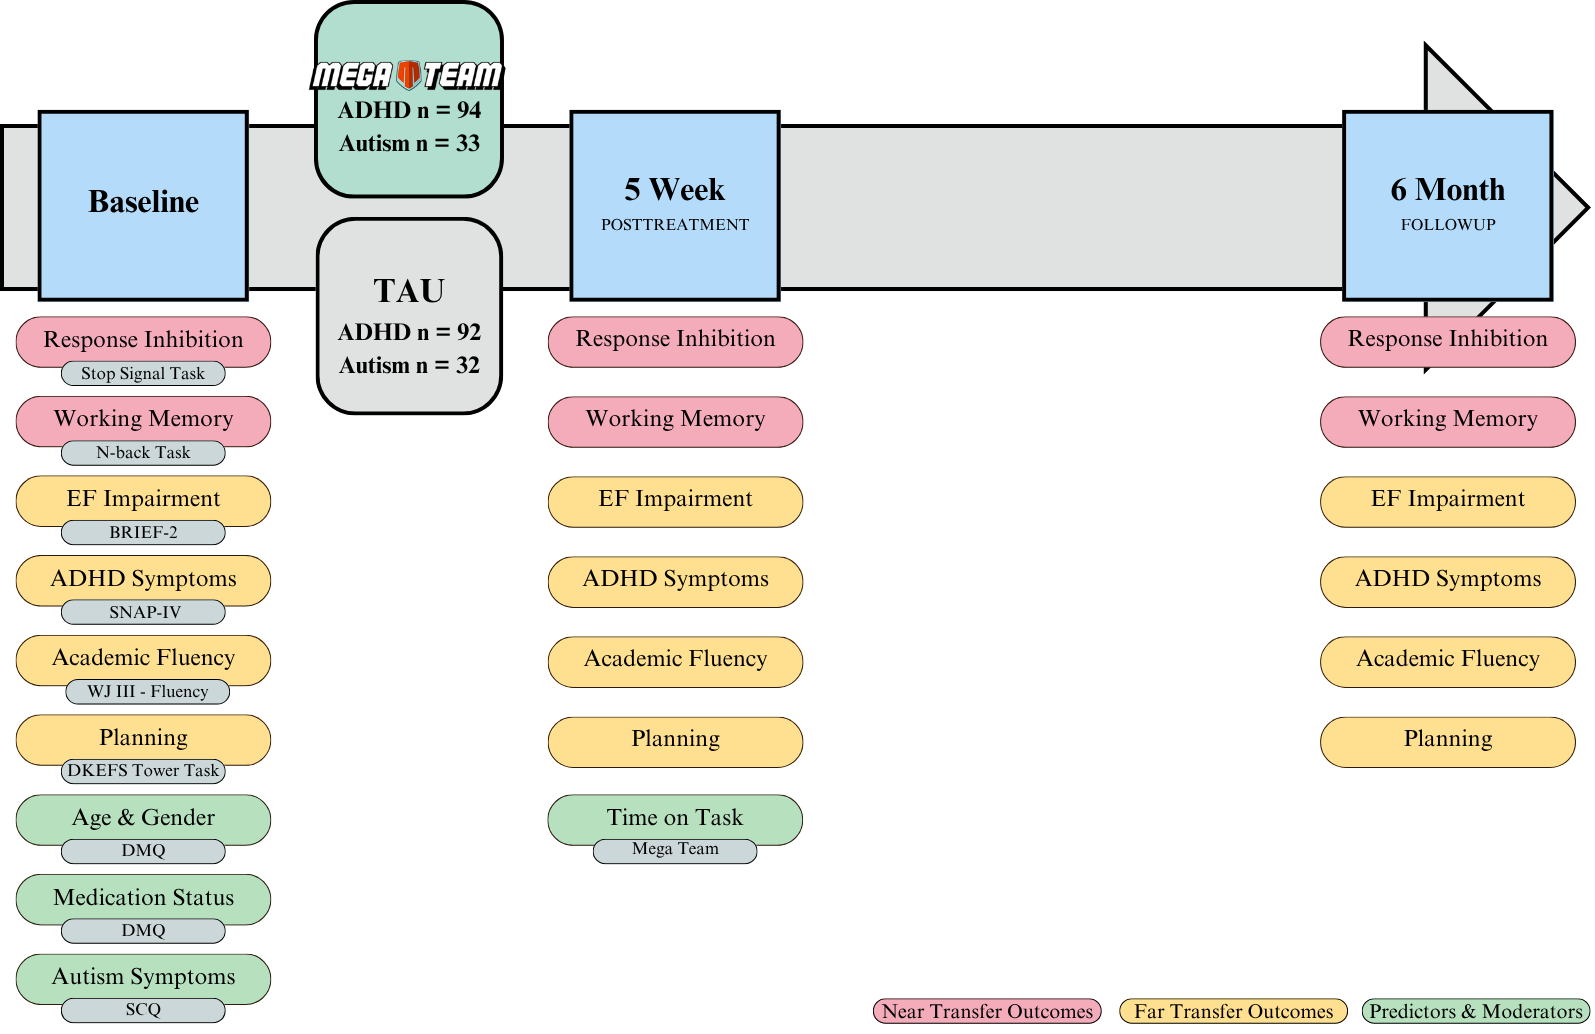
\includegraphics[keepaspectratio]{visitschematic.png}}

}

\end{figure}%

\section{Intervention}\label{intervention}

The Mega Team intervention trains response inhibition and working
memory. There are four minigames in Mega Team. Two minigames are played
on a laptop and two are played on a tablet. On each device, one game
trains response inhibition and the other trains working memory. Ideally
the games are collectively played for a total of 15 minutes per day,
five days per week, for five weeks, alternating between laptop and
tablet minigames with equal time spent on each minigame. The minigames
are adaptive so that the difficulty level is adjusted automatically and
dynamically to match the participant's ability while they play to remain
appropriately challenging. In the laptop minigames participants play as
various superhero characters dodging obstacles and collecting gems to
save other members of their superhero team (see
Figure~\ref{fig-megateam}). In the tablet minigames participants play
the role of a ninja battling different types of robots to beat each
level. In the response inhibition minigames participants are asked to
intermittently withhold their speeded response when a stop signal is
randomly presented and in the working memory minigames participants
progress in the game by indicating whether the picture on the screen
matches one presented previously. There is one minigame for each skill
on the laptop and on the tablet. Participants in the treatment group are
instructed to play all four minigames equally during the training
period. After the baseline assessment tasks were completed, participants
who were randomized to the treatment group were trained on how to play
the games. Parents were additionally provided with picture-based
instructions for reference and contact information of an unblinded
research assistant who could assist them with game-related questions.
Participants were incentivized to play daily using a training tracker on
which they used stickers to mark the days they played to earn a gift
card at their post-treatment visit.

\begin{figure}

\caption{\label{fig-megateam}Mega Team games}

\begin{minipage}{0.50\linewidth}
\subcaption{\label{}Response inhibition training task}

\pandocbounded{
\includegraphics[keepaspectratio]{actiondash.png}}

\end{minipage}%
%
\begin{minipage}{0.50\linewidth}
\subcaption{\label{}Working memory training task}

\pandocbounded{
\includegraphics[keepaspectratio]{dangerdive.png}}

\end{minipage}%

\end{figure}%

\section{Analysis}\label{analysis}

Data were screened for validity to check that certain thresholds were
met to indicate the task was completed accurately with a minimum
proportion of responses. An invalid Stop Signal Task administration
contained any of the following: fewer than 36 go trials, fewer than 12
stop trials, PSI less than 0.15 or greater than 0.85, greater than nine
non-responses, greater than two pre-pushes on stop trials, SSRT less
than 50 milliseconds (see supplemental materials in Schachar et al.,
2023). An invalid N-back task contained any of the following: target
accuracy greater than non-target accuracy plus twenty-eight, or fewer
than five target trials (e.g. Plas et al., 2016). Invalid administration
of tasks were excluded. Rates of invalid administrations collapsed
across all time points were not significantly different between the
treatment and TAU groups. Where multiple valid administrations were
collected at one study visit (due to technological issues), the first
administration was used to minimize the impact of fatigue on outcomes.
Raw scores for measures were used where possible as the current study
examined intra-individual change, and normed scores would limit the
ability to detect smaller changes.

Analyses were conducted in R {[}R version 4.4.1; R Core Team (2024){]}
on a machine using a Windows 11 64-bit operating system. Analyses were
run separately on the ADHD and autism diagnosis groups and used an
intention to treat principle. To examine the individual factors that
predict outcomes after Mega Team training, multiple linear regression
analyses were used. The fixed factor was treatment group (either Mega
Team or TAU). The outcomes were change scores after 5 weeks and after 6
months on Stop Signal Task SSRT, 1-back target accuracy, 2-back target
accuracy, BRIEF-2 GEC, SNAP total sum, Tower Task total achievement
score, and an academic fluency composite created from the Woodcock
Johnson's reading, math, and writing fluency standard scores. Means and
standard deviations of outcomes are presented in
Table~\ref{tbl-adhdoutcomes} for the ADHD group and
Table~\ref{tbl-asdoutcomes} for the autistic group. For the ADHD group,
the predictors and moderators tested were age, gender, stimulant
medication use, baseline ADHD symptoms, baseline autism traits, baseline
response inhibition, baseline working memory, baseline daily EF
impairment, and time on task over the course of treatment. In the autism
group predictors and moderators tested were baseline ADHD symptoms,
baseline autism traits, baseline response inhibition, baseline working
memory, and time on task over the course of treatment. The models
included interactions by randomization group on the predictors which
allowed confirmation that the results specifically reflect significance
in response to treatment (Mattes \& Roheger, 2020). The default lm
function listwise deletion was applied to missing data for complete case
analysis which is the most common approach (Bell et al., 2014). All
predictors were entered into each linear regression model together for a
given outcome to determine significance in the overall model and examine
the significance of individual predictors.

Predictor variables were checked for multicollinearity prior to
inclusion in the regression models. All baseline variable pairs returned
R2 \textless{} 0.8 resulting in a variance inflation factor of less than
5 (Kim et al., 2019) confirming no impact of multicollinearity on
results. Regression model diagnostics showed all assumptions necessary
for linear regression models were met. Diagnostic plots showed linearity
of data, normality of residuals, homogeneity of residual variance, and
independence of residual error terms in all models.

Significant predictors that displayed a pattern of results that could
not be distinguished from a potential regression to the mean were not
interpreted as meaningful significant predictors. Given the multiple
comparisons, Bonferroni correction was applied to adjust significance
threshold to reduce potential for false positives (i.e., Type I error).
The corrected significance value for the 14 models for the ADHD group
was p \textless{} 0.0035 (0.05/14) and the 6 for the autism group was
0.008 (0.05/6).

\begin{table}

\caption{\label{tbl-adhdoutcomes}ADHD Outcome Measures}

\centering{

\centering
\begin{threeparttable}
\resizebox{\ifdim\width>\linewidth\linewidth\else\width\fi}{!}{
\begin{tabular}{lcccccc}
\toprule
\multicolumn{1}{c}{ } & \multicolumn{2}{c}{\textbf{Baseline}} & \multicolumn{2}{c}{\textbf{5 Week Visit}} & \multicolumn{2}{c}{\textbf{6 Month Visit}} \\
\cmidrule(l{3pt}r{3pt}){2-3} \cmidrule(l{3pt}r{3pt}){4-5} \cmidrule(l{3pt}r{3pt}){6-7}
\textbf{Characteristic} & \makecell[c]{\textbf{Mega Team}\ \ \\N = 94} & \makecell[c]{\textbf{TAU}\ \ \\N = 92} & \makecell[c]{\textbf{Mega Team}\ \ \\N = 91} & \makecell[c]{\textbf{TAU}\ \ \\N = 84} & \makecell[c]{\textbf{Mega Team}\ \ \\N = 85} & \makecell[c]{\textbf{TAU}\ \ \\N = 84}\\
\midrule
SSRT & 375 (153) & 360 (137) & 306 (100) & 352 (188) & 294 (79) & 317 (157)\\
1-back Target Accuracy & 64 (20) & 60 (20) & 60 (24) & 62 (21) & 69 (21) & 66 (21)\\
2-back Target Accuracy & 43 (20) & 39 (16) & 37 (21) & 40 (22) & 47 (22) & 47 (21)\\
BRIEF2-GEC & 135 (19) & 139 (18) & 129 (19) & 137 (17) & 128 (21) & 138 (18)\\
SNAP Total & 34 (9) & 35 (9) & 29 (10) & 32 (9) & 29 (10) & 34 (10)\\
Fluency Composite & 85 (14) & 84 (14) & 86 (15) & 86 (16) & 87 (15) & 86 (14)\\
Total Achievement Score & 13.8 (3.6) & 13.5 (3.6) & 16.5 (3.2) & 16.2 (3.6) & 17.11 (2.95) & 17.46 (3.07)\\
\bottomrule
\end{tabular}}
\begin{tablenotes}[para]
\item \textit{Note: } 
\item M (SD); TAU: Treatment as Usual; SSRT: Stop Signal Reaction Time, BRIEF2-GEC: BRIEF2 Global Executive Composite
\end{tablenotes}
\end{threeparttable}

}

\end{table}%

\begin{table}

\caption{\label{tbl-asdoutcomes}Autism Outcome Measures}

\centering{

\centering
\begin{threeparttable}
\resizebox{\ifdim\width>\linewidth\linewidth\else\width\fi}{!}{
\begin{tabular}{lcccccc}
\toprule
\multicolumn{1}{c}{ } & \multicolumn{2}{c}{\textbf{Baseline}} & \multicolumn{2}{c}{\textbf{5 Week Visit}} & \multicolumn{2}{c}{\textbf{6 Month Visit}} \\
\cmidrule(l{3pt}r{3pt}){2-3} \cmidrule(l{3pt}r{3pt}){4-5} \cmidrule(l{3pt}r{3pt}){6-7}
\textbf{Characteristic} & \makecell[c]{\textbf{Mega Team}\ \ \\N = 33} & \makecell[c]{\textbf{TAU}\ \ \\N = 32} & \makecell[c]{\textbf{Mega Team}\ \ \\N = 29} & \makecell[c]{\textbf{TAU}\ \ \\N = 28} & \makecell[c]{\textbf{Mega Team}\ \ \\N = 26} & \makecell[c]{\textbf{TAU}\ \ \\N = 30}\\
\midrule
SSRT & 322 (171) & 436 (228) & 310 (112) & 392 (203) & 276 (84) & 289 (117)\\
1-back Target Accuracy & 61 (22) & 56 (20) & 61 (24) & 56 (20) & 67 (22) & 62 (22)\\
BRIEF2-GEC & 129 (26) & 141 (22) & 124 (24) & 135 (26) & 129 (25) & 138 (18)\\
\bottomrule
\end{tabular}}
\begin{tablenotes}[para]
\item \textit{Note: } 
\item M (SD); TAU: Treatment as Usual; SSRT: Stop Signal Reaction Time
\end{tablenotes}
\end{threeparttable}

}

\end{table}%

\bookmarksetup{startatroot}

\chapter{Results}\label{results}

\section{ADHD Group}\label{adhd-group}

\subsection{Baseline Factors Related to Change in Response
Inhibition}\label{baseline-factors-related-to-change-in-response-inhibition}

A multiple linear regression model for change in response inhibition
after 5 weeks of intervention with all the predictors (age, gender,
baseline response inhibition, working memory, EF impairment, ADHD
symptoms, autism traits, stimulant medication use, and time on task)
entered revealed a significant model fit indicating that the baseline
characteristics entered predicted response to treatment, accounting for
45\% of the variance (F = 4.7, p \textless{} 0.001, R\textsuperscript{2}
= 0.45). Baseline response inhibition (\(\beta\) = -0.30, p = 0.02) and
baseline working memory (\(\beta\) = -0.40, p = 0.0014) predicted
improvement in response inhibition after 5 weeks regardless of treatment
group such that lower (i.e., worse) baseline response inhibition and
higher (i.e., better) baseline working memory (on the N-Back 1-back
condition) predicted greater improvement after 5 weeks. Additionally,
the model showed a significant interaction effect of baseline response
inhibition by randomization group moderating change in response
inhibition at 5 weeks post-treatment (\(\beta\) = -0.65, p = 0.01),
ruling out the potential for regression to the mean explaining the
result.

This result showed that lower (i.e., worse) baseline response inhibition
was associated with a larger improvement in the Mega Team treatment
group than in the TAU control group in response inhibition after 5 weeks
of treatment. No other factors were significant predictors or moderators
of change in response inhibition after 5 weeks of treatment (see
Table~\ref{tbl-beta1}).

A multiple linear regression model for change in response inhibition at
6 month follow-up with all predictors entered showed a significant model
fit indicating that the baseline characteristics entered predicted
response to treatment, accounting for 55\% of the variance (F = 6.7, p
\textless{} 0.001, R\textsuperscript{2} = 0.55). Gender predicted
improvement in response inhibition regardless of treatment group such
that girls improved more after 6 months compared to boys (\(\beta\) =
0.20, p = 0.01). Baseline response inhibition (\(\beta\) = -0.60, p
\textless{} 0.001) and baseline working memory (N-back 1-back condition
only) (\(\beta\) = -0.40, p = 0.0011) predicted improvement in response
inhibition at 6 month follow-up regardless of treatment group, such that
lower (i.e., worse) baseline response inhibition and higher (i.e.,
better) baseline working memory (1-back) predicted greater improvement
at 6 month follow-up. Additionally, there was a significant interaction
effect of baseline working memory (1-back) by randomization group
moderating change in response inhibition (\(\beta\) = 0.91, p = 0.013),
such that in the TAU control group greater (i.e., better) baseline
working memory was associated with more improvement in response
inhibition compared to those in the Mega Team treatment group. No other
baseline factors were significant predictors or moderators of change in
response inhibition at 6 month follow-up.

\subsection{Baseline Factors in Change in Working
Memory}\label{baseline-factors-in-change-in-working-memory}

A multiple linear regression model for change in working memory (1-back
condition of the N-back) after treatment with all baseline predictors
entered revealed a significant model fit indicating baseline
characteristics entered predicted change in working memory accounting
for 32\% of the variance (F = 2.9, p \textless{} 0.001,
R\textsuperscript{2} = 0.32). Lower (i.e., weaker) baseline working
memory (1-back) predicted greater improvement in working memory (1-back)
after 5 weeks regardless of treatment group (\(\beta\) = -0.60, p
\textless{} 0.001). Additionally, time on task was a significant
predictor of change in working memory after 5 weeks of treatment
(\(\beta\) = 0.46, p = 0.037), such that greater time on task during
treatment was associated with greater improvement in working memory
after 5 weeks of treatment. No other individual baseline factors were
significant predictors or moderators of change in working memory after 5
weeks of treatment.

The overall multiple linear regression model for change in 1-back
working memory at 6 month follow-up with all baseline predictors entered
significantly predicted change in working memory accounting for 25\% of
the variance (F = 2, p = 0.014, R\textsuperscript{2} = 0.25); however
this finding did not maintain significance after Bonferroni correction
(p \textless{} 0.0035).

The overall multiple linear regression model for change in 2-back
working memory after 5 weeks of treatment with all baseline predictors
entered revealed a significant model fit which predicted 35\% of the
variance (F = 3.2,p \textless{} 0.001, R\textsuperscript{2} = 0.35).
Lower (i.e., weaker) baseline 2-back working memory predicted more
improvement on 2-back regardless of treatment group at 5 weeks
post-treatment (\(\beta\) = -0.40, p = 0.003). No other variables
predicted improvement, and none were significant moderators of change in
working memory (2-back task) at post-treatment.

At 6 month follow-up the multiple linear regression model for change in
2-back working memory revealed a significant model fit such that it
predicted 38\% of the variance (F = 3.5, p \textless{} 0.001,
R\textsuperscript{2} = 0.38). Similar to post-treatment, lower (i.e.,
weaker) baseline 2-back working memory predicted more improvement at 6
month follow-up regardless of treatment group (\(\beta\) = -0.60, p
\textless{} 0.001). Additionally, there was a significant interaction
effect of baseline 1-back working memory by randomization group
which\,moderated change in 2-back working memory at 6 month follow-up
(\(\beta\) = 1.3, p = 0.0024), such that higher (i.e., better) baseline
1-back accuracy was associated with more improvement in the treatment
group but not in the TAU group. No other factors were significant
predictors or moderators of 2-back working memory change at 6 month
follow-up.

\subsection{Baseline Factors in Change in ADHD
Symptoms}\label{baseline-factors-in-change-in-adhd-symptoms}

A multiple linear regression model predicting change in ADHD symptoms
after 5 weeks of training was significant overall and predicted 30\% of
the variance (F = 2.7, p \textless{} 0.001, R\textsuperscript{2} = 0.3)
and after 6 month follow-up predicting 35\% of the variance (F = 3.1, p
\textless{} 0.001, R\textsuperscript{2} = 0.35). At both time points,
lower baseline ADHD symptoms predicted greater improvement regardless of
treatment group: \(\beta\) = -0.70, p \textless{} 0.001, 6 months:
\(\beta\) = -0.50, p \textless{} 0.001). Additionally, at both time
points lower baseline EF impairment predicted greater improvement in
ADHD symptoms regardless of treatment group (\(\beta\) = -0.50, p
\textless{} 0.001, 6 months: \(\beta\) = -0.40, p = 0.005). No variables
moderated the relationship by treatment. See Table~\ref{tbl-beta2} for
results.

\subsection{Non-Significant Results}\label{non-significant-results}

A multiple linear regression with all predictors entered did not
significantly predict change in planning at 5 weeks post-treatment (F =
0.97, p = 0.5, R\textsuperscript{2} = 0.14) or at 6 month follow-up (F =
0.81, p = 0.69, R\textsuperscript{2} = 0.12) or predict academic fluency
at 5 weeks post-treatment (F = 0.96, p = 0.51, R\textsuperscript{2} =
0.16) or at 6 month follow-up. See Table~\ref{tbl-beta3} for results.

A multiple linear regression with all predictors entered did not
significantly predict change in EF impairment after 5 weeks of training
(F = 1.1, p = 0.33, R\textsuperscript{2} = 0.15) or at 6 month follow-up
(F = 1.9, p = 0.02, R\textsuperscript{2} = 0.24). See
Table~\ref{tbl-beta2} for results.

\begin{landscape}

\begin{table}

\caption{\label{tbl-beta1}Multiple Linear Regression Model Results
Predicting Response Inhibition and Working Memory in ADHD group}

\centering{

\centering
\begin{threeparttable}
\resizebox{\ifdim\width>\linewidth\linewidth\else\width\fi}{!}{
\begin{tabular}{lcccccccccccc}
\toprule
\multicolumn{1}{c}{Predictors} & \multicolumn{12}{c}{Outcomes} \\
\cmidrule(l{3pt}r{3pt}){1-1} \cmidrule(l{3pt}r{3pt}){2-13}
\multicolumn{1}{c}{ } & \multicolumn{2}{c}{\makecell[c]{\textbf{Δ SSRT 5 Week} \\F = 4.7* \\R² = 0.45}} & \multicolumn{2}{c}{\makecell[c]{\textbf{Δ SSRT 6 Month} \\F = 6.7* \\R² = 0.55}} & \multicolumn{2}{c}{\makecell[c]{\textbf{Δ 1-back 5 Week} \\F = 2.9* \\R² = 0.32}} & \multicolumn{2}{c}{\makecell[c]{\textbf{Δ 1-back 6 Month} \\F = 2 \\R² = 0.25}} & \multicolumn{2}{c}{\makecell[c]{\textbf{Δ 2-back 5 Week} \\F = 3.2* \\R² = 0.35}} & \multicolumn{2}{c}{\makecell[c]{\textbf{Δ 2-back 6 Month} \\F = 3.5* \\R² = 0.38}} \\
\cmidrule(l{3pt}r{3pt}){2-3} \cmidrule(l{3pt}r{3pt}){4-5} \cmidrule(l{3pt}r{3pt}){6-7} \cmidrule(l{3pt}r{3pt}){8-9} \cmidrule(l{3pt}r{3pt}){10-11} \cmidrule(l{3pt}r{3pt}){12-13}
 & $\beta$ & \textit{p} & $\beta$ & \textit{p} & $\beta$ & \textit{p} & $\beta$ & \textit{p} & $\beta$ & \textit{p} & $\beta$ & \textit{p}\\
\midrule
Stimulants & 0.14 & 0.5 & -0.18 & 0.4 & 0.23 & 0.3 & -0.04 & 0.9 & -0.29 & 0.2 & 0.18 & 0.4\\
Treatment Group & 0.15 & 0.3 & -0.15 & 0.9 & -1.0 & 0.066 & -0.12 & 0.4 & -0.93 & 0.4 & -0.25 & 0.4\\
SNAP Total & 0.16 & 0.2 & 0.19 & 0.11 & -0.03 & 0.8 & 0.11 & 0.5 & 0.03 & 0.8 & 0.10 & 0.5\\
SCQ Score & 0.13 & 0.2 & 0.10 & 0.3 & -0.03 & 0.8 & -0.02 & >0.9 & -0.12 & 0.3 & -0.21 & 0.071\\
SSRT & -0.30 & \textbf{0.022} & -0.65 & \textbf{<0.001} & -0.12 & 0.4 & -0.17 & 0.3 & -0.17 & 0.2 & -0.20 & 0.12\\
Target Accuracy (1-back) & -0.40 & \textbf{0.001} & -0.38 & \textbf{0.001} & -0.56 & \textbf{<0.001} & -0.59 & \textbf{<0.001} & 0.15 & 0.2 & 0.05 & 0.7\\
Target Accuracy (2-back) & 0.06 & 0.6 & -0.02 & 0.9 & 0.15 & 0.3 & 0.02 & 0.9 & -0.43 & \textbf{0.003} & -0.55 & \textbf{<0.001}\\
BRIEF-2 GEC & -0.11 & 0.5 & -0.12 & 0.4 & 0.01 & >0.9 & -0.23 & 0.2 & -0.08 & 0.6 & -0.10 & 0.5\\
Age & 0.21 & 0.066 & -0.04 & 0.7 & -0.08 & 0.5 & 0.29 & \textbf{0.034} & 0.22 & 0.063 & 0.19 & 0.12\\
Gender & 0.02 & >0.9 & 0.59 & \textbf{0.011} & 0.31 & 0.2 & -0.14 & 0.6 & -0.09 & 0.7 & 0.10 & 0.7\\
Time on task & -0.15 & 0.5 & -0.05 & 0.8 & 0.46 & \textbf{0.037} & 0.02 & >0.9 & 0.17 & 0.5 & 0.07 & 0.7\\
Stimulants * Treatment Group & -0.16 & 0.6 & 0.43 & 0.11 & -0.10 & 0.7 & 0.17 & 0.6 & 0.45 & 0.2 & -0.04 & >0.9\\
Treatment Group * SNAP Total & 0.05 & 0.8 & 0.01 & >0.9 & -0.20 & 0.4 & 0.01 & >0.9 & 0.09 & 0.7 & 0.25 & 0.3\\
Treatment Group * SCQ Score & -0.24 & 0.14 & -0.13 & 0.4 & -0.11 & 0.5 & -0.12 & 0.5 & -0.02 & >0.9 & 0.01 & >0.9\\
Treatment Group * SSRT & -0.43 & \textbf{0.010} & -0.19 & 0.2 & 0.10 & 0.6 & 0.09 & 0.7 & 0.24 & 0.2 & 0.00 & >0.9\\
Treatment Group * Target Accuracy (1-back) & 0.22 & 0.2 & 0.43 & \textbf{0.013} & 0.10 & 0.6 & 0.23 & 0.3 & 0.27 & 0.2 & 0.61 & \textbf{0.002}\\
Treatment Group * Target Accuracy (2-back) & -0.06 & 0.7 & -0.14 & 0.4 & -0.06 & 0.8 & -0.10 & 0.6 & -0.27 & 0.15 & -0.19 & 0.3\\
Treatment Group * BRIEF-2 GEC & -0.06 & 0.8 & -0.06 & 0.8 & 0.10 & 0.7 & 0.26 & 0.3 & -0.15 & 0.5 & -0.13 & 0.6\\
Treatment Group * Age & -0.11 & 0.5 & -0.03 & 0.9 & 0.33 & 0.076 & -0.19 & 0.3 & 0.05 & 0.8 & -0.07 & 0.7\\
Treatment Group * Gender & 0.04 & 0.9 & -0.53 & 0.11 & -0.54 & 0.13 & 0.00 & >0.9 & -0.03 & >0.9 & -0.21 & 0.6\\
\bottomrule
\end{tabular}}
\begin{tablenotes}[para]
\item \textit{Note: } 
\item SSRT - Stop Signal Reaction Time. *\textit{p}-value < 0.0035 (Bonferroni corrected); Bold p-value < 0.05.
\end{tablenotes}
\end{threeparttable}

}

\end{table}%

\begin{table}

\caption{\label{tbl-beta2}Multiple Linear Regression Model Results
Predicting EF Impairment and ADHD Symptoms in ADHD group}

\centering{

\centering
\begin{threeparttable}
\resizebox{\ifdim\width>\linewidth\linewidth\else\width\fi}{!}{
\begin{tabular}{lcccccccc}
\toprule
\multicolumn{1}{c}{Predictors} & \multicolumn{8}{c}{Outcomes} \\
\cmidrule(l{3pt}r{3pt}){1-1} \cmidrule(l{3pt}r{3pt}){2-9}
\multicolumn{1}{c}{ } & \multicolumn{2}{c}{\makecell[c]{\textbf{Δ BRIEF2-GEC 5 Week} \\F = 1.1 \\R² = 0.15}} & \multicolumn{2}{c}{\makecell[c]{\textbf{Δ BRIEF2-GEC 6 Month} \\F = 1.9 \\R² = 0.24}} & \multicolumn{2}{c}{\makecell[c]{\textbf{Δ SNAP-IV Total 5 Week} \\F = 2.7* \\R² = 0.3}} & \multicolumn{2}{c}{\makecell[c]{\textbf{Δ SNAP-IV Total 6 Month} \\F = 3.1* \\R² = 0.35}} \\
\cmidrule(l{3pt}r{3pt}){2-3} \cmidrule(l{3pt}r{3pt}){4-5} \cmidrule(l{3pt}r{3pt}){6-7} \cmidrule(l{3pt}r{3pt}){8-9}
 & $\beta$ & \textit{p} & $\beta$ & \textit{p} & $\beta$ & \textit{p} & $\beta$ & \textit{p}\\
\midrule
Stimulants & -0.01 & >0.9 & -0.21 & 0.4 & -0.04 & 0.9 & -0.19 & 0.4\\
Treatment Group & 0.33 & 0.8 & -0.20 & 0.3 & 0.13 & 0.4 & -0.66 & 0.7\\
SNAP Total & -0.04 & 0.8 & 0.01 & >0.9 & -0.75 & \textbf{<0.001} & -0.49 & \textbf{<0.001}\\
SCQ Score & -0.05 & 0.7 & -0.02 & 0.9 & -0.03 & 0.8 & 0.03 & 0.8\\
SSRT & 0.18 & 0.2 & 0.12 & 0.4 & -0.05 & 0.7 & 0.11 & 0.4\\
Target Accuracy (1-back) & -0.04 & 0.8 & 0.08 & 0.6 & -0.03 & 0.8 & 0.04 & 0.8\\
Target Accuracy (2-back) & -0.16 & 0.3 & -0.10 & 0.5 & -0.01 & >0.9 & 0.00 & >0.9\\
BRIEF-2 GEC & -0.22 & 0.2 & -0.16 & 0.3 & 0.54 & \textbf{<0.001} & 0.45 & \textbf{0.005}\\
Age & 0.04 & 0.8 & -0.23 & 0.084 & -0.05 & 0.7 & -0.21 & 0.10\\
Gender & 0.10 & 0.7 & -0.04 & 0.9 & -0.44 & 0.085 & 0.21 & 0.4\\
Time on task & -0.14 & 0.6 & -0.21 & 0.4 & -0.18 & 0.4 & 0.19 & 0.4\\
Stimulants * Treatment Group & -0.45 & 0.2 & 0.21 & 0.5 & 0.05 & 0.9 & 0.10 & 0.8\\
Treatment Group * SNAP Total & 0.01 & >0.9 & -0.13 & 0.6 & 0.09 & 0.7 & -0.21 & 0.4\\
Treatment Group * SCQ Score & 0.08 & 0.7 & -0.03 & 0.9 & 0.15 & 0.4 & -0.27 & 0.13\\
Treatment Group * SSRT & -0.28 & 0.2 & -0.26 & 0.2 & 0.01 & >0.9 & -0.13 & 0.4\\
Treatment Group * Target Accuracy (1-back) & 0.12 & 0.6 & -0.32 & 0.14 & 0.02 & >0.9 & -0.17 & 0.4\\
Treatment Group * Target Accuracy (2-back) & 0.03 & >0.9 & 0.15 & 0.5 & 0.08 & 0.7 & 0.14 & 0.5\\
Treatment Group * BRIEF-2 GEC & 0.00 & >0.9 & -0.05 & 0.8 & -0.21 & 0.4 & 0.24 & 0.3\\
Treatment Group * Age & 0.14 & 0.5 & 0.01 & >0.9 & -0.10 & 0.6 & -0.21 & 0.3\\
Treatment Group * Gender & -0.26 & 0.5 & 0.07 & 0.9 & 0.23 & 0.5 & -0.30 & 0.4\\
\bottomrule
\end{tabular}}
\begin{tablenotes}[para]
\item \textit{Note: } 
\item SSRT - Stop Signal Reaction Time. *p-value < 0.0035 (Bonferroni corrected); Bold p-value < 0.05
\end{tablenotes}
\end{threeparttable}

}

\end{table}%

\begin{table}

\caption{\label{tbl-beta3}Multiple Linear Regression Model Results
Predicting Planning and Fluency in ADHD group}

\centering{

\centering
\begin{threeparttable}
\resizebox{\ifdim\width>\linewidth\linewidth\else\width\fi}{!}{
\begin{tabular}{lcccccccc}
\toprule
\multicolumn{1}{c}{Predictors} & \multicolumn{8}{c}{Outcomes} \\
\cmidrule(l{3pt}r{3pt}){1-1} \cmidrule(l{3pt}r{3pt}){2-9}
\multicolumn{1}{c}{ } & \multicolumn{2}{c}{\makecell[c]{\textbf{Δ TAS 5 Week} \\F = 0.97 \\R² = 0.14}} & \multicolumn{2}{c}{\makecell[c]{\textbf{Δ TAS 6 Month} \\F = 0.81 \\R² = 0.12}} & \multicolumn{2}{c}{\makecell[c]{\textbf{Δ Fluency 5 Week} \\F = 0.96 \\R² = 0.16}} & \multicolumn{2}{c}{\makecell[c]{\textbf{Δ Fluency 6 Month} \\F = 0.45 \\R² = 0.086}} \\
\cmidrule(l{3pt}r{3pt}){2-3} \cmidrule(l{3pt}r{3pt}){4-5} \cmidrule(l{3pt}r{3pt}){6-7} \cmidrule(l{3pt}r{3pt}){8-9}
 & $\beta$ & \textit{p} & $\beta$ & \textit{p} & $\beta$ & \textit{p} & $\beta$ & \textit{p}\\
\midrule
Stimulants & 0.02 & >0.9 & -0.10 & 0.7 & -0.38 & 0.2 & -0.09 & 0.8\\
Treatment Group & -0.98 & 0.3 & -0.32 & 0.9 & -0.50 & 0.068 & 0.17 & 0.6\\
SNAP Total & -0.37 & \textbf{0.018} & -0.37 & \textbf{0.025} & -0.12 & 0.5 & 0.05 & 0.8\\
SCQ Score & 0.12 & 0.3 & -0.02 & 0.9 & -0.04 & 0.8 & -0.07 & 0.6\\
SSRT & 0.26 & 0.10 & 0.20 & 0.2 & 0.18 & 0.3 & -0.11 & 0.5\\
Target Accuracy (1-back) & -0.08 & 0.6 & 0.01 & >0.9 & 0.23 & 0.2 & 0.14 & 0.4\\
Target Accuracy (2-back) & 0.14 & 0.4 & -0.04 & 0.8 & 0.26 & 0.2 & -0.26 & 0.2\\
BRIEF-2 GEC & 0.33 & 0.070 & 0.33 & 0.072 & 0.13 & 0.6 & 0.15 & 0.5\\
Age & -0.06 & 0.7 & -0.08 & 0.6 & 0.14 & 0.4 & 0.12 & 0.5\\
Gender & -0.03 & >0.9 & -0.10 & 0.7 & -0.09 & 0.8 & 0.16 & 0.6\\
Time on task & 0.45 & 0.072 & -0.03 & >0.9 & 0.11 & 0.7 & -0.07 & 0.8\\
Stimulants * Treatment Group & 0.10 & 0.8 & 0.06 & 0.9 & 0.35 & 0.4 & 0.03 & >0.9\\
Treatment Group * SNAP Total & 0.58 & \textbf{0.022} & 0.23 & 0.4 & -0.11 & 0.7 & -0.02 & >0.9\\
Treatment Group * SCQ Score & -0.13 & 0.5 & 0.11 & 0.6 & -0.04 & 0.9 & 0.12 & 0.6\\
Treatment Group * SSRT & -0.26 & 0.2 & -0.10 & 0.6 & -0.17 & 0.5 & 0.06 & 0.8\\
Treatment Group * Target Accuracy (1-back) & 0.21 & 0.4 & -0.14 & 0.5 & -0.47 & 0.059 & -0.15 & 0.6\\
Treatment Group * Target Accuracy (2-back) & -0.08 & 0.7 & 0.25 & 0.3 & -0.27 & 0.3 & 0.25 & 0.3\\
Treatment Group * BRIEF-2 GEC & -0.55 & \textbf{0.031} & -0.23 & 0.4 & -0.19 & 0.5 & -0.30 & 0.4\\
Treatment Group * Age & -0.12 & 0.6 & 0.15 & 0.5 & -0.07 & 0.8 & 0.12 & 0.6\\
Treatment Group * Gender & 0.19 & 0.6 & 0.38 & 0.4 & 0.06 & >0.9 & -0.48 & 0.3\\
\bottomrule
\end{tabular}}
\begin{tablenotes}[para]
\item \textit{Note: } 
\item SSRT: Stop Signal Reaction Time; TAS: Total Achievement Score (Tower Task). *p-value < 0.0035 (Bonferroni corrected); Bold p-value < 0.05
\end{tablenotes}
\end{threeparttable}

}

\end{table}%

\end{landscape}

\section{Autism Group}\label{autism-group}

A multiple linear regression model with all predictors entered (baseline
response inhibition, working memory, ADHD symptoms, autism symptoms, and
time on task) significantly predicted improvement in response inhibition
at post-treatment (F = 2.4, p = 0.027, R\textsuperscript{2} = 0.38) and
at 6 month follow-up (F = 10, p \textless{} 0.001, R\textsuperscript{2}
= 0.74). Baseline response inhibition was a significant predictor of
improvement in response inhibition across both groups at post-treatment
(β = -0.6, p = 0.0024) and at 6 month follow-up (β = -0.6, p \textless{}
0.001). No other individual factors were significant predictors or
moderators of response inhibition at 5 weeks or 6 months. See
Table~\ref{tbl-beta-asd} for results.

Multiple linear regression models with all the predictors did not
predict improvement in working memory (1-back) after 5 weeks
post-treatment (F = 1.4, p = 0.2, R\textsuperscript{2} = 0.26) or at 6
months follow-up (F = 1.3, p = 0.25, R\textsuperscript{2} = 0.26).

Finally, a multiple linear regression model with all predictors entered
predicting EF impairment was not significant at post-treatment (F =
0.86, p = 0.59, R\textsuperscript{2} = 0.2). However, at 6 months
follow-up the multiple linear regression model significantly predicted
improvement in daily EF impairment (F = 2.1, p = 0.044,
R\textsuperscript{2} = 0.4); however, no individual variables
significantly predicted or moderated response.

However, after applying Bonferroni correction to adjust for multiple
comparisons (threshold p \textless{} 0.008) only the model predicting
response inhibition at 6 month follow-up remained significant.

\begin{landscape}

\begin{table}

\caption{\label{tbl-beta-asd}Multiple Linear Regression Model Results
Predicting Response Inhibition, Working Memory, and EF Impairment in
Autistic group}

\centering{

\centering
\begin{threeparttable}
\resizebox{\ifdim\width>\linewidth\linewidth\else\width\fi}{!}{
\begin{tabular}{lcccccccccccc}
\toprule
\multicolumn{1}{c}{Predictors} & \multicolumn{12}{c}{Outcomes} \\
\cmidrule(l{3pt}r{3pt}){1-1} \cmidrule(l{3pt}r{3pt}){2-13}
\multicolumn{1}{c}{ } & \multicolumn{2}{c}{\makecell[c]{\textbf{Δ SSRT 5 Week} \\F = 2.4 \\R² = 0.38}} & \multicolumn{2}{c}{\makecell[c]{\textbf{Δ SSRT 6 Month} \\F = 10 \\R² = 0.74}} & \multicolumn{2}{c}{\makecell[c]{\textbf{Δ 1-back 5 Week} \\F = 1.4 \\R² = 0.26}} & \multicolumn{2}{c}{\makecell[c]{\textbf{Δ 1-back 6 Month} \\F = 1.3 \\R² = 0.26}} & \multicolumn{2}{c}{\makecell[c]{\textbf{Δ BRIEF-2 5 Week} \\F = 0.86 \\R² = 0.2}} & \multicolumn{2}{c}{\makecell[c]{\textbf{Δ BRIEF-2 6 Month} \\F = 2.1 \\R² = 0.4}} \\
\cmidrule(l{3pt}r{3pt}){2-3} \cmidrule(l{3pt}r{3pt}){4-5} \cmidrule(l{3pt}r{3pt}){6-7} \cmidrule(l{3pt}r{3pt}){8-9} \cmidrule(l{3pt}r{3pt}){10-11} \cmidrule(l{3pt}r{3pt}){12-13}
 & $\beta$ & \textit{p} & $\beta$ & \textit{p} & $\beta$ & \textit{p} & $\beta$ & \textit{p} & $\beta$ & \textit{p} & $\beta$ & \textit{p}\\
\midrule
SCQ Score & -0.10 & 0.6 & 0.03 & 0.8 & -0.12 & 0.5 & -0.05 & 0.8 & -0.22 & 0.3 & -0.06 & 0.7\\
Treatment Group & -0.21 & >0.9 & -0.97 & 0.3 & -1.3 & 0.14 & 0.64 & 0.8 & 1.3 & 0.5 & 1.4 & 0.8\\
SNAP Total & -0.40 & \textbf{0.033} & -0.22 & 0.092 & -0.02 & >0.9 & -0.18 & 0.4 & 0.20 & 0.7 & 0.38 & 0.3\\
SSRT & -0.60 & \textbf{0.002} & -0.80 & \textbf{<0.001} & 0.02 & >0.9 & -0.11 & 0.6 & -0.16 & 0.5 & 0.12 & 0.6\\
Target Accuracy (1-back) & 0.22 & 0.3 & 0.10 & 0.4 & -0.34 & 0.2 & -0.37 & 0.12 & 0.12 & 0.6 & -0.01 & >0.9\\
Time on task & -0.05 & >0.9 & 0.51 & 0.3 & 0.86 & 0.10 & -0.26 & 0.7 & -0.83 & 0.13 & -0.84 & 0.15\\
SCQ Score * Treatment Group & -0.09 & 0.8 & 0.21 & 0.4 & 0.57 & 0.14 & 0.64 & 0.13 & 0.50 & 0.2 & 0.49 & 0.2\\
Treatment Group * SNAP Total & 0.45 & 0.14 & 0.13 & 0.5 & -0.34 & 0.3 & -0.33 & 0.3 & -0.54 & 0.3 & -0.44 & 0.4\\
Treatment Group * SSRT & -0.04 & >0.9 & 0.02 & >0.9 & 0.36 & 0.4 & 0.04 & >0.9 & -0.22 & 0.6 & -0.26 & 0.6\\
Treatment Group * Target Accuracy (1-back) & -0.30 & 0.3 & -0.06 & 0.8 & 0.17 & 0.6 & 0.12 & 0.7 & -0.15 & 0.7 & -0.25 & 0.4\\
BRIEF-2 GEC &  &  &  &  &  &  &  &  & -0.23 & 0.7 & -0.87 & 0.10\\
Treatment Group * BRIEF-2 GEC &  &  &  &  &  &  &  &  & 0.04 & >0.9 & 0.32 & 0.6\\
\bottomrule
\end{tabular}}
\begin{tablenotes}[para]
\item \textit{Note: } 
\item SSRT: Stop Signal Reaction Time; TAU - Treatment as Usual; *p-value < 0.008 (Bonferroni corrected); Bold p-value < 0.05
\end{tablenotes}
\end{threeparttable}

}

\end{table}%

\end{landscape}

\bookmarksetup{startatroot}

\chapter{Discussion}\label{discussion}

\section{Main Findings}\label{main-findings}

This project aimed to explore the impact of individual factors on
response to EF training given the heterogeneity of previous study
results examining efficacy of EF training in ADHD and autistic children.
In particular, the current study explored whether participants' baseline
demographic, EF and clinical characteristics, as well as their
engagement during EF training (as indexed by time spent training) were
predictors and moderators of response to EF training. Age, gender,
response inhibition, working memory, EF impairment, ADHD symptoms,
autism traits, stimulant medication use, and time on task were used as
predictors and moderators of response. The overall goal of the study was
to explore how these individual factors were associated with response to
Mega Team immediately after training (5 weeks) and at 6 month follow-up
on measures of near transfer of training (response inhibition and
working memory) and far transfer of training (EF impairment, ADHD
symptoms, planning, and fluency) in a sample of 186 ADHD and 67 autistic
children. Existing work on computerized EF training interventions have
shown that EF training is moderated by age (Cao et al., 2020), sex
(Flannery et al., 2024), ADHD symptom severity (Davis et al., 2018),
ADHD subtype (van der Donk et al., 2020), autism traits (de Vries et
al., 2018), baseline working memory (van der Donk et al., 2020),
baseline response inhibition (Dovis et al., 2019), and medication use
(Holmes et al., 2010; van der Donk et al., 2020). However, these
previous results were often not replicated or were not corrected for
multiple comparisons.

Results of the current study revealed several significant predictors and
moderators of response to EF training in the ADHD participants but not
in the autistic participants. In the ADHD participants, baseline working
memory and gender were significant predictors of improvement in response
inhibition and baseline EF impairment was a significant predictor of
improvement in ADHD symptoms over time regardless of treatment group. In
addition, baseline response inhibition and baseline working memory were
significantly moderated by treatment group on indices of change in
response inhibition and working memory. Finally, time on task was a
significant predictor of improvement in working memory across both
groups.

\subsection{ADHD Group}\label{adhd-group-1}

\textbf{Age \& Gender}

In the current study, age was not a significant predictor or moderator
of EF training related improvement at either time point for any outcome.
This is contrary to findings from a review looking across diagnosis
groups (typically developing, ADHD, fragile X, and learning
disabilities) including participants with an age range of 3-12 years old
that showed an age effect whereby younger children benefited more from
computerized EF training than older children (Cao et al., 2020).
Findings from the Westwood et al. (2023) review, however, did not show a
similar relationship in studies of 8-14 year old ADHD children only.
Given the rapid development of EFs in preschool ages (Reilly et al.,
2022), our sample of school aged children may not have a wide enough age
range to observe age-related influences in EF training related outcomes
that may exist earlier in development.

A review of the literature describes minimal group level differences in
EF performance by gender across ages, but identifies some differences in
development of EFs in children by gender, for example typically
developing girls outperforming boys in an attention task at 8-10 years
old whereas no gender differences are observed in adolescence (Grissom
\& Reyes, 2019). In the current analysis, gender predicted improvement
in response inhibition at 6 month follow-up irrespective of treatment
group such that girls improved more than boys. The results are in line
with a recent analysis showing female participants improved more than
male participants in attention scores following attention training
(Flannery et al., 2024), which did not distinguish the presence of a
treatment specific effect over and above an effect of time. Altogether,
the current results suggest that there are differences in development of
EFs in childhood by gender, but no reported differences in response to
training.

\textbf{EF Characteristics}

Results from the current study support previous findings showing a
relationship between baseline response inhibition and improvement in
response inhibition (near transfer) as a function of EF training (Dovis
et al., 2019). Specifically, we found that that receiving EF training
resulted in significantly greater improvement for participants with
relatively worse baseline response inhibition than ones who did not
receive EF training. This aligns with the theory that weaker baseline EF
leaves a greater capacity for improvement as described by Diamond \& Lee
(2011) otherwise known as a compensation effect. This pattern has been
observed in studies of working memory training (van der Donk et al.,
2020) and attention training (Davis et al., 2018), specifically when the
EF being measured at baseline (e.g.\,low working memory) matched the
type of EF training (e.g.\,working memory). However, this same pattern
was not observed when using a composite of multiple EF skills as a
predictor and moderator (Minder et al., 2019), suggesting that a broad
metric of multiple EF skills may not be sensitive enough to pick up this
relationship. Results from the current study are consistent with
previous research showing that worse baseline ability on a specific
skill predicted greater improvement on that same skill when the training
content matched that deficit pre treatment.

On the other hand, we observed an interaction by treatment group effect
such that higher (better) baseline 1-back working memory performance was
associated with greater improvement in 2-back working memory in the Mega
Team treatment group but not in the TAU control group at 6 month follow
up which is contrary to the findings of van der Donk et al. (2020). This
finding is notable given that results from the Mega Team RCT did not
show significant group-level (i.e., Mega Team vs TAU) differences in
2-back working memory within the same time frame (Cheung et al., in
prep), indicating the presence of a unique treatment response in a
subset of the group. A potential explanation for this discrepancy may be
the differences in the type of training between the studies. Whereas van
der Donk et al. (2020) administered only working memory training
(CogMed) for a longer total session length in their computerized EF
training condition, Mega Team training was composed of both response
inhibition and working memory training and for a shorter total session
length. This resulted in an average of 1125 minutes of total working
memory training per participant in the van der Donk et al. (2020) study
and an average of 187.5 minutes of total working memory training per
participant in our study over a 5 week training period in both. In
general, working memory training doses vary within the literature (see
review Robledo-Castro et al., 2023) with some evidence that higher doses
of working memory training could be more effective than lower doses
(Alloway et al., 2013; Liu et al., 2024). Our results may indicate that
in the context of a lower dose of training, individuals with relatively
stronger baseline working memory may improve more with training and
perhaps that a higher dose of working memory training than what was
completed in our study may be required to benefit participants with
lower working memory at pre-treatment. This dose-related pattern of
improvement has been shown in a sample of typically developing older
adults (Matysiak et al., 2019).

Our results also show significant cross-EF (i.e.\,working memory to
response inhibition) prediction of response to training at both outcome
time points, and significant moderation by treatment group at 6 month
follow-up. Higher (better) baseline 1-back working memory predicted
greater improvement in response inhibition at 5 weeks post-treatment and
at 6 month follow-up overall across treatment groups. More specifically
at 6 month follow-up the participants in the Mega Team group with
stronger baseline working memory no longer had an advantage over weaker
baseline working memory participants as seen in the control group. To
date, other studies have not observed this cross-EF moderation effect
(Dovis et al., 2019; Minder et al., 2019; van der Donk et al., 2020).
This finding may be explained by the relationship between working memory
and response inhibition. First, stronger working memory may predict
subsequent improvement in response inhibition because both skills rely
on overlapping brain regions necessary across EFs such as the
fronto-parietal and cingulo-opercular networks (Friedman \& Robbins,
2022) and may be the result of better developed shared brain regions at
baseline across participants (both Mega Team and TAU groups) which
result in more improvement as a function of time. However, this
explanation would be best supported with results showing a stronger
baseline in \emph{either} working memory or response inhibition predicts
improvement in the other skill, which is not seen in our study. An
alternative explanation may be based in theoretical models of EFs which
propose the various ways working memory, response inhibition, and other
EF skills may be interrelated and rely on one another in ADHD
individuals. For example, some models propose underlying skill deficits
that may explain impairments associated with ADHD such as response
inhibition (Barkley, 1997) or working memory (Rapport et al., 2008). Our
results align with theoretical models proposing working memory as the
key underlying deficit explaining other difficulties in ADHD as we found
that improvement in response inhibition at 5 weeks post treatment and at
6 month follow-up was associated with better developed working memory at
baseline across Mega Team and TAU groups. It may be that response
inhibition development over time in ADHD children may be reliant on
earlier working memory ability. Then in response to Mega Team training,
this relationship is negated at 6 month follow-up, so baseline working
memory no longer explained improvements in response inhibition,
indicating all levels of baseline working memory could benefit from Mega
Team Training.

Parent rating of EF impairment via the BRIEF-2 rating scale at baseline
predicted greater improvement in ADHD symptoms over time across both
Mega Team and TAU control groups at 5 weeks post-treatment and at 6
month follow-up. Findings from the literature suggest that EF impairment
as rated on the BRIEF-2 is correlated with ratings of ADHD severity
(Jacobson et al., 2020). Results align with expectations of the
developmental relationship between EF impairment and ADHD symptoms
across participants (Mega Team and TAU) over time. However, this
relationship was not moderated by treatment group (Mega Team or TAU) at
any time point and baseline daily EF impairment scores did not predict
or moderate any other outcome. Minder et al. (2019) showed that lower
parent rated daily EF impairment at baseline was associated with greater
improvement in EF impairment after 12 weeks of EF training than in a
higher parent rated impairment subgroup, however they did not compare
these outcomes with those of a control group's making it difficult to
distinguish the presence of a treatment-specific change in EF
impairment. There is no other existing literature that we know of
exploring EF impairment as a moderator of response to EF training in
ADHD children. Despite non-significant relationships with training
outcomes, ratings of daily EF related impairments warrant further
investigation as a factor in EF training response. Baseline EF
impairment may relate to adherence to treatment protocol especially in
interventions with high EF demands in engaging with intervention or
minimal rewards or external motivators. Future work should consider the
relationship of baseline EF functioning to other training-related
factors beyond training outcomes.

\textbf{Clinical Characteristics}

Clinical characteristics (e.g.\,ADHD symptoms, autism traits, stimulant
medication use) were not significant predictors or moderators of
improvement at either time point for any outcome in the current study.
Existing literature has demonstrated a significant effect for ADHD
severity (Davis et al., 2018), subtype (van der Donk et al., 2020),
autism traits (de Vries et al., 2018), and stimulant medication status
(Holmes et al., 2010; van der Donk et al., 2020) on response to EF
training, however, these findings are inconsistent (e.g., no effect of
ADHD severity or stimulant medication (Jones et al., 2018), no effect of
autism traits (Kirk et al., 2021)). It is possible that measurement or
sample differences explain inconsistent results across studies. In the
present study, parent rated clinical characteristics were used as
predictors and moderators, whereas studies with significant ADHD
severity and subtype used outcomes from diagnostic interviews and
psychological report reviews. In the existing literature, autism traits
were significant only in an autistic sample, not in another condition
(i.e.\,intellectual and developmental disorders) (Kirk et al., 2021),
which may explain why they were not a significant predictor of treatment
response in our ADHD participants.

\textbf{Time on Task}

In the present study, greater time on task during EF training predicted
greater improvement on working memory at 5 weeks post-treatment. These
findings reflect the importance of engagement with training as
individuals who played more practiced their EFs more and therefore
improved more at 5 weeks post-treatment. This result is notable within
the context of the overall efficacy results showing no significant
differences in group-level (Mega Team vs TAU) performance (Cheung et
al., in prep). Previous research has shown evidence of greater efficacy
of working memory training because of intervention dosage. This has been
observed when dosage was randomly assigned (Alloway et al., 2013) and
when dosage of training varied due to participants' motivation to train
(Jaeggi et al., 2014). Despite the initially straightforward nature of
this relationship, the components underlying a metric like time on task
are complex. In the present study, all participants were instructed to
play the minigames for the same amount of time so the variation in time
played is reflective of individual differences like motivation to play
or the influence of caregivers' EFs on facilitating training (e.g.,
scheduling). Existing literature indicates there are differences in
reward processing and motivation in individuals with neurodevelopmental
disorders versus typically developing children suggesting overall
deficits in reward processing with variation within and between groups
(Dichter et al., 2012; Kohls et al., 2014). In line with the literature,
Mega Team games were designed based on children and youth's interests
(e.g.\,variety of games) and efforts were made to support motivation to
play with weekly tracker and salience of associated rewards. However,
motivation to play and interest in the games were not directly analyzed
so future work should investigate whether games and rewards used during
Mega Team training were perceived as motivating and rewarding. Existing
literature also suggests that the relationship between parent and child
EF skills fits within a complex multifaceted framework composed of
genetic and socialization factors (Bridgett et al., 2015). Based on
this, efforts were made to minimize demands on caregiver EFs to engage
with intervention and incorporate the games into their existing
lifestyles as much as possible (e.g.,\,focusing on portability of
training with minimal reliance on WiFi, providing weekly phone reminders
and check ins). Caregivers' EF ability and level of involvement in
facilitating the training were not captured in this study and future
research exploring their impact on time on task may be beneficial in
understanding these relationships. Notably, many of the design elements
described above were a result of engagement with youth and parents,
supporting the use of patient-oriented research approaches in digital
intervention design (described further in Cheung et al., in prep). Given
the significance of time on task in the present study, future research
should aim to better understand barriers and facilitators to engaging
with videogame-based EF training, which could impact time spent training
by children and thereby impact treatment outcomes.

\subsection{Autism Group}\label{autism-group-1}

The small sample size (N = 67) of autistic children in our sample may
have influenced the non-significant findings in the autistic group.
Additionally, despite randomization to treatment condition, the Mega
Team and TAU groups had some significantly different baseline scores
(e.g., baseline response inhibition) potentially restricting the range
of scores in each group and interfering with the ability to detect
relationships. None of the factors explored were significant in
influencing training outcomes for the autism group, conflicting with
findings reported by de Vries et al. (2018) showing autism traits were a
significant predictor. This may reflect that the predictors and
moderators selected were not specific enough to the autism phenotype as
de Vries et al. (2018) found that baseline flexibility was a significant
predictor in training outcomes. Individual factors predicting response
to treatment in the autistic participants may need to be approached
differently to be more specific to the presentation - for example
capturing additional EF skills such as including shifting or examining
the severity and variation associated with restricted, repetitive,
behaviours and interests in addition to social communication.

\subsection{Summary}\label{summary}

Overall results highlight the importance of baseline EF profiles and
time on task in near transfer of EF training. There were significant
factors in the context of both significant overall group-level Mega Team
versus TAU differences (e.g.~response inhibition) and in the context of
no overall differences in response (e.g.~1-back working memory at 5
weeks). This avenue of work has the potential to clarify the key
ingredients influencing transfer of training. None of the factors
explored were significant moderators of far transfer of training (as
indexed by parent rated daily EF impairment, ADHD symptoms, planning,
and fluency). Different factors were significant at 5 weeks post
treatment (response inhibition and time on task) and at 6 month
follow-up (response inhibition and working memory). Baseline response
inhibition and time on task during training were significant factors
associated with response at 5 weeks post-treatment in improvement in
response inhibition and working memory, whereas baseline working memory
was a significant factor associated with ongoing benefit or maintenance
of gains at 6 month follow-up in improvements in working memory and
response inhibition. Age, gender, and clinical characteristics were not
meaningful moderators of response.

\section{Strengths \& Limitations}\label{strengths-limitations}

A major strength of this project is the patient-oriented approach. Mega
Team minigames and study protocols were designed together with families
and youth with lived and living experiences. Iterative feedback was
incorporated during pilot phases to optimize child interest and
enjoyment in games and convenience and practicality for caregivers.
Given the significance of time on task as a predictor of improvement on
working memory, future studies should prioritize family and youth
perspectives in intervention designs to increase engagement. Efforts to
increase enjoyment and convenience are likely to increase accessibility
by for example, minimizing demands on parent EFs to facilitate training.
Another strength of the current study was the multi-EF training design
as there are relatively fewer studies exploring multi-EF training
compared to single-EF training (Westwood et al., 2023). Existing work on
predictors and moderators of response in multi-skill training is very
limited. In addition, the inclusion of a 6 month follow-up to observe
predictors and moderators of longer-term benefits or maintenance of
effects was another positive of the current study. Several significant
relationships appeared at 6 month follow-up that were not present
immediately at 5-weeks post-treatment. Evidence from a meta-analysis
suggests that within the limited trials looking at overall efficacy at
follow-up, there were a range of significant improvements maintained and
some small effects emerged only at follow-up (Westwood et al., 2023).
Inclusion of a follow-up in understanding predictors and moderators of
response clarifies factors associated with not only immediate response
but also later consolidation and maintenance of gains. Finally, though
not significant, the inclusion of autistic participants is an important
step in developing a better understanding of the effects of computerized
EF training across overlapping diagnostic categories like ADHD and
autism.

Results also need to be considered in the context of study limitations.
First, when interpreting the parent questionnaire results, it should be
noted that parents were aware of their child's treatment group. This
knowledge may have biased results on parent-reported outcomes (daily EF
impairment and ADHD symptoms) due to expectation of improvement and
masked the presence of moderators of response. Future studies should
seek to incorporate an active sham condition (e.g., games with no EF
load) so that parents and children are blinded to minimize inflation of
results. Second, data collection for the current study spanned the
COVID-19 pandemic which impacted this research like many others during
this period. Data was collected from 2018 to 2023 with a subset of
participants experiencing delayed follow-up assessments due to lockdowns
with 14 participants having post-treatment visits more than 8 weeks
after baseline and 10 participants having follow-up visits more than 9
months after baseline. Participant retention was prioritized over strict
adherence to post-treatment and follow-up visit schedule given the
unprecedented circumstances. Future studies may benefit from
incorporating a sensitivity analysis to better understand COVID-19
related impacts on results. Finally, the autism participant group was
ultimately quite small and reflected a fairly narrow slice of the
population. These participants had average IQ and were primarily verbal.
Despite a lack of variation in these characteristics, autism is known to
be quite heterogeneous in other aspects as well and so the small sample
size may not have captured enough of a range of characteristics to
identify potential predictors and moderators. Despite randomization,
autistic participants in the Mega Team group had significantly stronger
response inhibition performance at baseline than the TAU control group.
Given these limitations, results may not accurately capture predictors
or moderators of response in autistic individuals. As computerized EF
training in autism is currently a fairly small area of study, it would
be beneficial for future research efforts to incorporate predictors and
moderators of response while exploring overall efficacy.

\section{Implications \& Future
Directions}\label{implications-future-directions}

Theoretical implications of this work are relevant to EF models of
impairment in ADHD and compensation versus magnification effects in EF
skills. Different models have been proposed to explain the roles of
various EF skills within ADHD related impairment (for example summary
table within Kofler et al., 2024) and these findings support the idea
that working memory may be a core deficit (Rapport et al., 2008)
explaining some of the other difficulties observed in ADHD. A better
understanding of the relationship between the EF deficits observed in
neurodevelopmental disorders is key for improving intervention design.
The second theoretical implication addresses hypotheses of how
individual differences in EF skills change in response to intervention.
Literature is mixed with competing hypotheses suggesting either a
compensation effect (i.e., lower baseline EF have greater capacity for
improvement) (e.g. Diamond \& Lee, 2011) or a magnification effect
(i.e., higher baseline EFs are able to benefit more from intervention)
(e.g., Von Bastian \& Oberauer, 2014). We saw evidence for both types of
effects in different baseline EF skills and so it remains unknown if the
variation could be the result of different skills responding differently
to intervention, baseline ability interacting with training intensity,
or some other difference in the components of intervention. Further work
is needed to identify potential patterns in how baseline EF abilities
respond to intervention.

Methodological implications of these results support the inclusion of
follow-up appointments in assessments of EF training. In the limited
work following up after treatment there is some evidence of improvements
emerging only at mid to long term follow-up (Westwood et al., 2023). Our
results support the presence of baseline characteristics that may be
relevant factors in continued development of skills or retention of
training gains at follow-up.

A clinical implication of these findings is the lack of explanation for
what factors influence far transfer of computerized EF training as there
were no significant moderators of far transfer. The unexplained
heterogeneity in far transfer results supports the caution around
computerized EF training as a clinically meaningful intervention option
at this time (Westwood et al., 2023). Heterogeneity in far transfer
results in computerized EF training warrants further work with blinded
trial designs to understand predictors and moderators of response.

Another clinical implication is that lower baseline EF impairment
(better EF) predicted improvement in ADHD symptoms regardless of group.
This relationship adds to our understanding of how real-world EF
impairment relates to changes in ADHD symptoms over time. In line with
the established gap between EF task performance and EF related
impairment (Toplak et al., 2013), performance-based EF tasks do not
predict later ADHD symptoms (Coghill et al., 2014) but parent ratings of
EF impairment do (Hawkey et al., 2018). Understanding the mechanisms
that translate EF skills to application in real-world settings is
essential to identifying factors associated with far transfer of
training.

In conclusion, the current study showed that near transfer of response
to EF training (as indexed by response inhibition and working memory
tasks) was associated with baseline EF characteristics and time spent
training but not with baseline clinical or demographic characteristics
in ADHD children. Personalizing EF training based on baseline EF
characteristics and developing interventions that are engaging may
enhance treatment results. EF training may be equally beneficial across
a range of clinical presentations as none of the clinical
characteristics measured in the current study (e.g., ADHD symptoms or
autism traits) were associated with near or far transfer of outcomes.
Relevant participant characteristics that are associated with far
transfer of training remain unknown. In addition, more work is needed to
identify potential characteristics associated with computerized EF
training responses in autistic children.

\bookmarksetup{startatroot}

\chapter*{References}\label{references}
\addcontentsline{toc}{chapter}{References}

\markboth{References}{References}

\phantomsection\label{refs}
\begin{CSLReferences}{1}{0}
\bibitem[\citeproctext]{ref-alabdulakareem2020}
Alabdulakareem, E., \& Jamjoom, M. (2020). Computer-assisted learning
for improving {ADHD} individuals' executive functions through gamified
interventions: {A} review. \emph{Entertainment Computing}, \emph{33},
100341. \url{https://doi.org/10.1016/j.entcom.2020.100341}

\bibitem[\citeproctext]{ref-alloway2013}
Alloway, T. P., Bibile, V., \& Lau, G. (2013). Computerized working
memory training: {Can} it lead to gains in cognitive skills in students?
\emph{Computers in Human Behavior}, \emph{29}(3), 632--638.
\url{https://doi.org/10.1016/j.chb.2012.10.023}

\bibitem[\citeproctext]{ref-americanpsychiatricassociation2022}
American Psychiatric Association. (2022). \emph{Diagnostic and
statistical manual of mental disorders : {DSM-5-TR}} (5th edition, text
revision.). American Psychiatric Association Publishing.
\url{https://doi/book/10.1176/appi.books.9780890425787}

\bibitem[\citeproctext]{ref-assari2021}
Assari, S. (2021). Emotional, behavioral, and cognitive correlates of
attention deficit and hyperactive disorder ({ADHD}) screening and
diagnosis history: {Sex}/gender differences. \emph{Journal of Neurology
\& Neuromedicine}, \emph{6}(1).
\url{https://doi.org/10.29245/2572.942X/2021/1.1278}

\bibitem[\citeproctext]{ref-ayano2023}
Ayano, G., Demelash, S., Gizachew, Y., Tsegay, L., \& Alati, R. (2023).
The global prevalence of attention deficit hyperactivity disorder in
children and adolescents: {An} umbrella review of meta-analyses.
\emph{Journal of Affective Disorders}, \emph{339}, 860--866.
\url{https://doi.org/10.1016/j.jad.2023.07.071}

\bibitem[\citeproctext]{ref-barkley1997}
Barkley, R. A. (1997). Behavioral inhibition, sustained attention, and
executive functions: Constructing a unifying theory of {ADHD}.
\emph{Psychological Bulletin}, \emph{121}(1), 65--94.
\url{https://doi.org/10.1037/0033-2909.121.1.65}

\bibitem[\citeproctext]{ref-bell2014}
Bell, M. L., Fiero, M., Horton, N. J., \& Hsu, C.-H. (2014). Handling
missing data in {RCTs}; a review of the top medical journals. \emph{BMC
Medical Research Methodology}, \emph{14}(1), 118.
\url{https://doi.org/10.1186/1471-2288-14-118}

\bibitem[\citeproctext]{ref-best2010}
Best, J. R., \& Miller, P. H. (2010). A developmental perspective on
executive function. \emph{Child Development}, \emph{81}(6), 1641--1660.
\url{https://doi.org/10.1111/j.1467-8624.2010.01499.x}

\bibitem[\citeproctext]{ref-bridgett2015}
Bridgett, D. J., Burt, N. M., Edwards, E. S., \& Deater-Deckard, K.
(2015). Intergenerational transmission of self-regulation: A
multidisciplinary review and integrative conceptual framework.
\emph{Psychological Bulletin}, \emph{141}(3), 602--654.
\url{https://doi.org/10.1037/a0038662}

\bibitem[\citeproctext]{ref-bussing2008}
Bussing, R., Fernandez, M., Harwood, M., Hou, W., Garvan, C. W.,
Swanson, J. M., \& Eyberg, S. M. (2008). Parent and teacher {SNAP-IV}
ratings of attention deficit/hyperactivity disorder symptoms:
{Psychometric} properties and normative ratings from a school district
sample. \emph{Assessment}, \emph{15}(3), 317--328.
\url{https://doi.org/10.1177/1073191107313888}

\bibitem[\citeproctext]{ref-cao2020}
Cao, Y., Huang, T., Huang, J., Xie, X., \& Wang, Y. (2020). Effects and
moderators of computer-based training on children's executive functions:
A systematic review and meta-analysis. \emph{Frontiers in Psychology},
\emph{11}, 580329. \url{https://doi.org/10.3389/fpsyg.2020.580329}

\bibitem[\citeproctext]{ref-chacko2014}
Chacko, A., Bedard, A. c., Marks, D. j., Feirsen, N., Uderman, J. z.,
Chimiklis, A., Rajwan, E., Cornwell, M., Anderson, L., Zwilling, A., \&
Ramon, M. (2014). A randomized clinical trial of {Cogmed Working Memory
Training} in school-age children with {ADHD}: A replication in a diverse
sample using a control condition. \emph{Journal of Child Psychology and
Psychiatry}, \emph{55}(3), 247--255.
\url{https://doi.org/10.1111/jcpp.12146}

\bibitem[\citeproctext]{ref-chandler2007}
Chandler, S., Charman, T., Baird, G., Simonoff, E., Loucas, T., Meldrum,
D., Scott, M., \& Pickles, A. (2007). Validation of the social
communication questionnaire in a population cohort of children with
autism spectrum disorders. \emph{Journal of the American Academy of
Child \& Adolescent Psychiatry}, \emph{46}(10), 1324--1332.
\url{https://doi.org/10.1097/chi.0b013e31812f7d8d}

\bibitem[\citeproctext]{ref-cheungRCT}
Cheung, T. C. K., Ram, N., Anagnostou, E., Ameis, S. H., Sananes, R.,
Bedard, A.-C., \& Crosbie, J. (in prep). \emph{Cognitive rehabilitation
({Mega Team}) and its effects on emotional and behavioural regulation in
{ADHD} and {ASD} children}.

\bibitem[\citeproctext]{ref-coghill2014}
Coghill, D. R., Hayward, D., Rhodes, S. M., Grimmer, C., \& Matthews, K.
(2014). A longitudinal examination of neuropsychological and clinical
functioning in boys with attention deficit hyperactivity disorder
({ADHD}): Improvements in executive functioning do not explain clinical
improvement. \emph{Psychological Medicine}, \emph{44}(5), 1087--1099.
\url{https://doi.org/10.1017/S0033291713001761}

\bibitem[\citeproctext]{ref-cortese2015}
Cortese, S., Ferrin, M., Brandeis, D., Buitelaar, J., Daley, D.,
Dittmann, R. W., Holtmann, M., Santosh, P., Stevenson, J., Stringaris,
A., Zuddas, A., \& Sonuga-Barke, E. J. S. (2015). Cognitive training for
attention-deficit/hyperactivity disorder: {Meta-analysis} of clinical
and neuropsychological outcomes from randomized controlled trials.
\emph{Journal of the American Academy of Child \& Adolescent
Psychiatry}, \emph{54}(3), 164--174.
\url{https://doi.org/10.1016/j.jaac.2014.12.010}

\bibitem[\citeproctext]{ref-davis2018}
Davis, N. O., Bower, J., \& Kollins, S. H. (2018). Proof-of-concept
study of an at-home, engaging, digital intervention for pediatric
{ADHD}. \emph{PloS One}, \emph{13}(1), e0189749.
\url{https://doi.org/10.1371/journal.pone.0189749}

\bibitem[\citeproctext]{ref-devries2015}
de Vries, M., Prins, P. J. M., Schmand, B. A., \& Geurts, H. M. (2015).
Working memory and cognitive flexibility-training for children with an
autism spectrum disorder: A randomized controlled trial. \emph{Journal
of Child Psychology and Psychiatry, and Allied Disciplines},
\emph{56}(5), 566--576. \url{https://doi.org/10.1111/jcpp.12324}

\bibitem[\citeproctext]{ref-devries2018}
de Vries, M., Verdam, M. G., Prins, P. J., Schmand, B. A., \& Geurts, H.
M. (2018). Exploring possible predictors and moderators of an executive
function training for children with an autism spectrum disorder.
\emph{Autism : The International Journal of Research and Practice},
\emph{22}(4), 440--449. \url{https://doi.org/10.1177/1362361316682622}

\bibitem[\citeproctext]{ref-delis2001}
Delis, D. C., Kaplan, E., \& Kramer, J. H. (2001). \emph{Delis-{Kaplan
Executive Function System}}.
\url{https://doi.apa.org/doi/10.1037/t15082-000}

\bibitem[\citeproctext]{ref-diamond2013}
Diamond, A. (2013). Executive functions. \emph{Annual Review of
Psychology}, \emph{64}, 135--168.
\url{https://doi.org/10.1146/annurev-psych-113011-143750}

\bibitem[\citeproctext]{ref-diamond2011}
Diamond, A., \& Lee, K. (2011). Interventions shown to aid executive
function development in children 4--12 years old. \emph{Science (New
York, N.Y.)}, \emph{333}(6045), 959--964.
\url{https://doi.org/10.1126/science.1204529}

\bibitem[\citeproctext]{ref-dichter2012}
Dichter, G. S., Damiano, C. A., \& Allen, J. A. (2012). Reward circuitry
dysfunction in psychiatric and neurodevelopmental disorders and genetic
syndromes: Animal models and clinical findings. \emph{Journal of
Neurodevelopmental Disorders}, \emph{4}(1), 19.
\url{https://doi.org/10.1186/1866-1955-4-19}

\bibitem[\citeproctext]{ref-dombrowski2015}
Dombrowski, S. C. (2015). Exploratory bifactor analysis of the {WJ-III}
achievement at school age via the schmid-leiman orthogonalization
procedure. \emph{Canadian Journal of School Psychology}, \emph{30}(1),
34--50. \url{https://doi.org/10.1177/0829573514560529}

\bibitem[\citeproctext]{ref-dovis2019}
Dovis, S., Maric, M., Prins, P. J. M., \& Van der Oord, S. (2019). Does
executive function capacity moderate the outcome of executive function
training in children with {ADHD}? \emph{ADHD Attention Deficit and
Hyperactivity Disorders}, \emph{11}(4), 445--460.
\url{https://doi.org/10.1007/s12402-019-00308-5}

\bibitem[\citeproctext]{ref-dovis2015}
Dovis, S., Oord, S. V. der, Wiers, R. W., \& Prins, P. J. M. (2015).
Improving executive functioning in children with {ADHD}: {Training}
multiple executive functions within the context of a computer game. {A}
randomized double-blind placebo controlled trial. \emph{PLOS ONE},
\emph{10}(4), e0121651.
\url{https://doi.org/10.1371/journal.pone.0121651}

\bibitem[\citeproctext]{ref-faraone2021}
Faraone, S. V., Banaschewski, T., Coghill, D., Zheng, Y., Biederman, J.,
Bellgrove, M. A., Newcorn, J. H., Gignac, M., Al Saud, N. M., Manor, I.,
Rohde, L. A., Yang, L., Cortese, S., Almagor, D., Stein, M. A., Albatti,
T. H., Aljoudi, H. F., Alqahtani, M. M. J., Asherson, P., \ldots{} Wang,
Y. (2021). The world federation of {ADHD} international consensus
statement: 208 evidence-based conclusions about the disorder.
\emph{Neuroscience \& Biobehavioral Reviews}, \emph{128}, 789--818.
\url{https://doi.org/10.1016/j.neubiorev.2021.01.022}

\bibitem[\citeproctext]{ref-flannery2024}
Flannery, J. E., Hinshaw, S. P., Kollins, S. H., \& Stamatis, C. A.
(2024). Secondary analyses of sex differences in attention improvements
across three clinical trials of a digital therapeutic in children,
adolescents, and adults with {ADHD}. \emph{BMC Public Health},
\emph{24}, 1195. \url{https://doi.org/10.1186/s12889-024-18597-5}

\bibitem[\citeproctext]{ref-french2024}
French, B., Nalbant, G., Wright, H., Sayal, K., Daley, D., Groom, M. J.,
Cassidy, S., \& Hall, C. L. (2024). The impacts associated with having
{ADHD}: An umbrella review. \emph{Frontiers in Psychiatry}, \emph{15}.
\url{https://doi.org/10.3389/fpsyt.2024.1343314}

\bibitem[\citeproctext]{ref-friedman2017}
Friedman, N. P., \& Miyake, A. (2017). Unity and diversity of executive
functions: {Individual} differences as a window on cognitive structure.
\emph{Cortex; a Journal Devoted to the Study of the Nervous System and
Behavior}, \emph{86}, 186--204.
\url{https://doi.org/10.1016/j.cortex.2016.04.023}

\bibitem[\citeproctext]{ref-friedman2022}
Friedman, N. P., \& Robbins, T. W. (2022). The role of prefrontal cortex
in cognitive control and executive function.
\emph{Neuropsychopharmacology : Official Publication of the American
College of Neuropsychopharmacology}, \emph{47}(1), 72--89.
\url{https://doi.org/10.1038/s41386-021-01132-0}

\bibitem[\citeproctext]{ref-gioia2000}
Gioia, G. A., Isquith, P. K., Guy, S. C., \& Kenworthy, L. (2000).
Behavior rating inventory of executive function. \emph{Child
Neuropsychology}, \emph{6}, 235--238.
https://doi.org/\url{http://dx.doi.org/10.1076/chin.6.3.235.3152}

\bibitem[\citeproctext]{ref-grissom2019}
Grissom, N. M., \& Reyes, T. M. (2019). Let's call the whole thing off:
Evaluating gender and sex differences in executive function.
\emph{Neuropsychopharmacology : Official Publication of the American
College of Neuropsychopharmacology}, \emph{44}(1), 86--96.
\url{https://doi.org/10.1038/s41386-018-0179-5}

\bibitem[\citeproctext]{ref-hasson2012}
Hasson, R., \& Fine, J. G. (2012). Gender differences among children
with {ADHD} on continuous performance tests: A meta-analytic review.
\emph{Journal of Attention Disorders}, \emph{16}(3), 190--198.
\url{https://doi.org/10.1177/1087054711427398}

\bibitem[\citeproctext]{ref-hawkey2018}
Hawkey, E. J., Tillman, R., Luby, J. L., \& Barch, D. M. (2018).
Preschool executive function predicts childhood resting-state functional
connectivity and attention-deficit/hyperactivity disorder and
depression. \emph{Biological Psychiatry: Cognitive Neuroscience and
Neuroimaging}, \emph{3}(11), 927--936.
\url{https://doi.org/10.1016/j.bpsc.2018.06.011}

\bibitem[\citeproctext]{ref-hendrickson2019}
Hendrickson, N. K., \& McCrimmon, A. W. (2019). Test review: {Behavior}
rating inventory of executive function®, second edition ({BRIEF}®2) by
gioia, {G}. {A}., isquith, {P}. {K}., guy, {S}. {C}., \& kenworthy, {L}.
\emph{Canadian Journal of School Psychology}, \emph{34}(1), 73--78.
\url{https://doi.org/10.1177/0829573518797762}

\bibitem[\citeproctext]{ref-hill2004}
Hill, E. L. (2004). Executive dysfunction in autism. \emph{Trends in
Cognitive Sciences}, \emph{8}(1), 26--32.
\url{https://doi.org/10.1016/j.tics.2003.11.003}

\bibitem[\citeproctext]{ref-holmes2010}
Holmes, J., Gathercole, S. E., Place, M., Dunning, D. L., Hilton, K. A.,
\& Elliott, J. G. (2010). Working memory deficits can be overcome:
{Impacts} of training and medication on working memory in children with
{ADHD}. \emph{Applied Cognitive Psychology}, \emph{24}(6), 827--836.
\url{https://doi.org/10.1002/acp.1589}

\bibitem[\citeproctext]{ref-ickowicz2006}
Ickowicz, A., Schachar, R. J., Sugarman, R., Chen, S. X., Millette, C.,
\& Cook, L. (2006). The parent interview for child symptoms: A
situation-specific clinical research interview for attention-deficit
hyperactivity and related disorders. \emph{Canadian Journal of
Psychiatry.}, \emph{51}(5), 325--328.
\url{https://doi.org/10.1177/070674370605100508}

\bibitem[\citeproctext]{ref-irby2013}
Irby, S. M., \& Floyd, R. G. (2013). Test review: {Wechsler} abbreviated
scale of intelligence, second edition. \emph{Canadian Journal of School
Psychology}, \emph{28}(3), 295--299.
\url{https://doi.org/10.1177/0829573513493982}

\bibitem[\citeproctext]{ref-jacobson2020}
Jacobson, L. A., Pritchard, A. E., Koriakin, T. A., Jones, K. E., \&
Mahone, E. M. (2020). Initial examination of the {BRIEF2} in clinically
referred children with and without {ADHD} symptoms. \emph{Journal of
Attention Disorders}, \emph{24}(12), 1775--1784.
\url{https://doi.org/10.1177/1087054716663632}

\bibitem[\citeproctext]{ref-jaeggi2014}
Jaeggi, S. M., Buschkuehl, M., Shah, P., \& Jonides, J. (2014). The role
of individual differences in cognitive training and transfer.
\emph{Memory \& Cognition}, \emph{42}(3), 464--480.
\url{https://doi.org/10.3758/s13421-013-0364-z}

\bibitem[\citeproctext]{ref-jones2018}
Jones, M. R., Katz, B., Buschkueh, M., Jaeggi, S. M., \& Shah, P.
(2018). Exploring n-back cognitive training for children with {ADHD}.
\emph{Journal of Attention Disorders}, 1087054718779230.
\url{https://doi.org/10.1177/1087054718779230}

\bibitem[\citeproctext]{ref-kim2019}
Kim, J., Gabriel, U., \& Gygax, P. (2019). Testing the effectiveness of
the {Internet-based} instrument {PsyToolkit}: {A} comparison between
web-based ({PsyToolkit}) and lab-based ({E-Prime} 3.0) measurements of
response choice and response time in a complex psycholinguistic task.
\emph{PLOS ONE}, \emph{14}(9), e0221802.
\url{https://doi.org/10.1371/journal.pone.0221802}

\bibitem[\citeproctext]{ref-kirk2021}
Kirk, H. E., Raber, A., Richmond, S., \& Cornish, K. M. (2021).
Examining potential predictors of attention training outcomes in
children with intellectual and developmental disorders. \emph{Journal of
Intellectual \& Developmental Disability}, \emph{46}(3), 197--203.
\url{https://doi.org/10.3109/13668250.2020.1821939}

\bibitem[\citeproctext]{ref-klingberg2002}
Klingberg, T., Forssberg, \& and Westerberg, H. (2002). Training of
working memory in children with {ADHD}. \emph{Journal of Clinical and
Experimental Neuropsychology}, \emph{24}(6), 781--791.
\url{https://doi.org/10.1076/jcen.24.6.781.8395}

\bibitem[\citeproctext]{ref-kofler2024}
Kofler, M. J., Soto, E. F., Singh, L. J., Harmon, S. L., Jaisle, E. M.,
Smith, J. N., Feeney, K. E., \& Musser, E. D. (2024). Executive function
deficits in attention-deficit/hyperactivity disorder and autism spectrum
disorder. \emph{Nature Reviews Psychology}, 1--19.
\url{https://doi.org/10.1038/s44159-024-00350-9}

\bibitem[\citeproctext]{ref-kohls2014}
Kohls, G., Thönessen, H., Bartley, G. K., Grossheinrich, N., Fink, G.
R., Herpertz-Dahlmann, B., \& Konrad, K. (2014). Differentiating neural
reward responsiveness in autism versus {ADHD}. \emph{Developmental
Cognitive Neuroscience}, \emph{10}, 104--116.
\url{https://doi.org/10.1016/j.dcn.2014.08.003}

\bibitem[\citeproctext]{ref-kollins2020}
Kollins, S. H., DeLoss, D. J., Cañadas, E., Lutz, J., Findling, R. L.,
Keefe, R. S. E., Epstein, J. N., Cutler, A. J., \& Faraone, S. V.
(2020). A novel digital intervention for actively reducing severity of
paediatric {ADHD} ({STARS-ADHD}): A randomised controlled trial.
\emph{The Lancet Digital Health}, \emph{2}(4), e168--e178.
\url{https://doi.org/10.1016/S2589-7500(20)30017-0}

\bibitem[\citeproctext]{ref-lambek2018}
Lambek, R., Sonuga-Barke, E., Tannock, R., Sørensen, A. V., Damm, D., \&
Thomsen, P. H. (2018). Are there distinct cognitive and motivational
sub-groups of children with {ADHD}? \emph{Psychological Medicine},
\emph{48}(10), 1722--1730.
\url{https://doi.org/10.1017/S0033291717003245}

\bibitem[\citeproctext]{ref-lebersfeld2021}
Lebersfeld, J. B., Swanson, M., Clesi, C. D., \& O'Kelley, S. E. (2021).
Systematic review and meta-analysis of the clinical utility of the
{ADOS-2} and the {ADI-r} in diagnosing autism spectrum disorders in
children. \emph{Journal of Autism and Developmental Disorders},
\emph{51}(11), 4101--4114.
\url{https://doi.org/10.1007/s10803-020-04839-z}

\bibitem[\citeproctext]{ref-liu2024}
Liu, L., Wang, H., Xing, Y., Zhang, Z., Zhang, Q., Dong, M., Ma, Z.,
Cai, L., Wang, X., \& Tang, Y. (2024). Dose--response relationship
between computerized cognitive training and cognitive improvement.
\emph{Npj Digital Medicine}, \emph{7}(1), 1--7.
\url{https://doi.org/10.1038/s41746-024-01210-9}

\bibitem[\citeproctext]{ref-logan1997}
Logan, G. D., Schachar, R. J., \& Tannock, R. (1997). Impulsivity and
inhibitory control. \emph{Psychological Science}, \emph{8}(1), 60--64.
\url{https://doi.org/10.1111/j.1467-9280.1997.tb00545.x}

\bibitem[\citeproctext]{ref-lord2020}
Lord, C., Brugha, T. S., Charman, T., Cusack, J., Dumas, G., Frazier,
T., Jones, E. J. H., Jones, R. M., Pickles, A., State, M. W., Taylor, J.
L., \& Veenstra-VanderWeele, J. (2020). Autism spectrum disorder.
\emph{Nature Reviews. Disease Primers}, \emph{6}(1), 5.
\url{https://doi.org/10.1038/s41572-019-0138-4}

\bibitem[\citeproctext]{ref-lord2012}
Lord, C., Rutter, M., DiLavore, P., Risi, S., Gotham, K., \& Bishop, S.
(2012). \emph{Diagnostic observation schedule, second edition ({ADOS-2})
manual (part {I}): {Modules} 1-4}. Western Psychological Services.

\bibitem[\citeproctext]{ref-luo2019}
Luo, Y., Weibman, D., Halperin, J. M., \& Li, X. (2019). A review of
heterogeneity in attention deficit/hyperactivity disorder ({ADHD}).
\emph{Frontiers in Human Neuroscience}, \emph{13}, 42.
\url{https://doi.org/10.3389/fnhum.2019.00042}

\bibitem[\citeproctext]{ref-masi2017}
Masi, A., DeMayo, M. M., Glozier, N., \& Guastella, A. J. (2017). An
overview of autism spectrum disorder, heterogeneity and treatment
options. \emph{Neuroscience Bulletin}, \emph{33}(2), 183--193.
\url{https://doi.org/10.1007/s12264-017-0100-y}

\bibitem[\citeproctext]{ref-mattes2020}
Mattes, A., \& Roheger, M. (2020). Nothing wrong about change: The
adequate choice of the dependent variable and design in prediction of
cognitive training success. \emph{BMC Medical Research Methodology},
\emph{20}(1), 296. \url{https://doi.org/10.1186/s12874-020-01176-8}

\bibitem[\citeproctext]{ref-matysiak2019}
Matysiak, O., Kroemeke, A., \& Brzezicka, A. (2019). Working memory
capacity as a predictor of cognitive training efficacy in the elderly
population. \emph{Frontiers in Aging Neuroscience}, \emph{11}, 126.
\url{https://doi.org/10.3389/fnagi.2019.00126}

\bibitem[\citeproctext]{ref-mcgrew2007}
McGrew, K., Woodcock, R., \& Schrank, K. (2007). \emph{Technical manual.
{Woodcock-Johnson III} normative update}. Riverside.

\bibitem[\citeproctext]{ref-medina2021}
Medina, R., Bouhaben, J., de Ramón, I., Cuesta, P., Antón-Toro, L.,
Pacios, J., Quintero, J., Ramos-Quiroga, J. A., \& Maestú, F. (2021).
Electrophysiological brain changes associated with cognitive improvement
in a pediatric attention deficit hyperactivity disorder digital
artificial intelligence-driven intervention: {Randomized} controlled
trial. \emph{Journal of Medical Internet Research}, \emph{23}(11),
e25466. \url{https://doi.org/10.2196/25466}

\bibitem[\citeproctext]{ref-minder2019}
Minder, F., Zuberer, A., Brandeis, D., \& Drechsler, R. (2019). Specific
effects of individualized cognitive training in children with
attention-deficit/hyperactivity disorder ({ADHD}): {The} role of
pre-training cognitive impairment and individual training performance.
\emph{Developmental Neurorehabilitation}, \emph{22}(6), 400--414.
\url{https://doi.org/10.1080/17518423.2019.1600064}

\bibitem[\citeproctext]{ref-owen2005}
Owen, A. M., McMillan, K. M., Laird, A. R., \& Bullmore, E. (2005).
N-back working memory paradigm: A meta-analysis of normative functional
neuroimaging studies. \emph{Human Brain Mapping}, \emph{25}(1), 46--59.
\url{https://doi.org/10.1002/hbm.20131}

\bibitem[\citeproctext]{ref-pasqualotto2021}
Pasqualotto, A., Mazzoni, N., Bentenuto, A., Mulè, A., Benso, F., \&
Venuti, P. (2021). Effects of cognitive training programs on executive
function in children and adolescents with autism spectrum disorder: A
systematic review. \emph{Brain Sciences}, \emph{11}(10), 1280.
\url{https://doi.org/10.3390/brainsci11101280}

\bibitem[\citeproctext]{ref-pettersson2019}
Pettersson, E., Lichtenstein, P., Larsson, H., Song, J., Agrawal, A.,
Børglum, A. D., Bulik, C. M., Daly, M. J., Davis, L. K., Demontis, D.,
Edenberg, H. J., Grove, J., Gelernter, J., Neale, B. M., Pardiñas, A.
F., Stahl, E., Walters, J. T. R., Walters, R., Sullivan, P. F., \ldots{}
Polderman, T. J. C. (2019). Genetic influences on eight psychiatric
disorders based on family data of 4 408 646 full and half-siblings, and
genetic data of 333 748 cases and controls. \emph{Psychological
Medicine}, \emph{49}(7), 1166--1173.
\url{https://doi.org/10.1017/S0033291718002039}

\bibitem[\citeproctext]{ref-vanderplas2016}
Plas, E. van der, Schachar, R. J., Hitzler, J., Crosbie, J., Guger, S.
L., Spiegler, B. J., Ito, S., \& Nieman, B. J. (2016). Brain structure,
working memory and response inhibition in childhood leukemia survivors.
\emph{Brain and Behavior}, \emph{7}(2), e00621.
\url{https://doi.org/10.1002/brb3.621}

\bibitem[\citeproctext]{ref-posar2019}
Posar, A., \& Visconti, P. (2019). Long-term outcome of autism spectrum
disorder. \emph{Turkish Archives of Pediatrics/Türk Pediatri Arşivi},
\emph{54}(4), 207--212.
\url{https://doi.org/10.14744/TurkPediatriArs.2019.16768}

\bibitem[\citeproctext]{ref-rcoreteam2024}
R Core Team. (2024). \emph{R: A language and environment for statistical
computing}. \url{https://www.R-project.org/}

\bibitem[\citeproctext]{ref-rapport2008}
Rapport, M. D., Alderson, R. M., Kofler, M. J., Sarver, D. E., Bolden,
J., \& Sims, V. (2008). Working memory deficits in boys with
attention-deficit/hyperactivity disorder ({ADHD}): The contribution of
central executive and subsystem processes. \emph{Journal of Abnormal
Child Psychology}, \emph{36}(6), 825--837.
\url{https://doi.org/10.1007/s10802-008-9215-y}

\bibitem[\citeproctext]{ref-reilly2022}
Reilly, S. E., Downer, J. T., \& Grimm, K. J. (2022). Developmental
trajectories of executive functions from preschool to kindergarten.
\emph{Developmental Science}, \emph{25}(5), e13236.
\url{https://doi.org/10.1111/desc.13236}

\bibitem[\citeproctext]{ref-roberts2016}
Roberts, G., Quach, J., Spencer-Smith, M., Anderson, P. J., Gathercole,
S., Gold, L., Sia, K.-L., Mensah, F., Rickards, F., Ainley, J., \& Wake,
M. (2016). Academic outcomes 2 years after working memory training for
children with low working memory: A randomized clinical trial.
\emph{JAMA Pediatrics}, \emph{170}(5), e154568.
\url{https://doi.org/10.1001/jamapediatrics.2015.4568}

\bibitem[\citeproctext]{ref-robledo-castro2023}
Robledo-Castro, C., Lerma-Castaño, P. R., \& Bonilla-Santos, G. (2023).
Effect of cognitive training programs based on computer systems on
executive functions in children with {ADHD}: A systematic review.
\emph{Journal of Attention Disorders}, \emph{27}(13), 1467--1487.
\url{https://doi.org/10.1177/10870547231187164}

\bibitem[\citeproctext]{ref-rong2021}
Rong, Y., Yang, C.-J., Jin, Y., \& Wang, Y. (2021). Prevalence of
attention-deficit/hyperactivity disorder in individuals with autism
spectrum disorder: {A} meta-analysis. \emph{Research in Autism Spectrum
Disorders}, \emph{83}, 101759.
\url{https://doi.org/10.1016/j.rasd.2021.101759}

\bibitem[\citeproctext]{ref-rutter2003}
Rutter, M., Bailey, A., \& Lord, C. (2003). \emph{The social
communication questionnaire: {Manual}}. Western Psychological Services.

\bibitem[\citeproctext]{ref-sadozai2024}
Sadozai, A. K., Sun, C., Demetriou, E. A., Lampit, A., Munro, M., Perry,
N., Boulton, K. A., \& Guastella, A. J. (2024). Executive function in
children with neurodevelopmental conditions: A systematic review and
meta-analysis. \emph{Nature Human Behaviour}, \emph{8}(12), 2357--2366.
\url{https://doi.org/10.1038/s41562-024-02000-9}

\bibitem[\citeproctext]{ref-schachar2023}
Schachar, R. J., Dupuis, A., Arnold, P. D., Anagnostou, E., Kelley, E.,
Georgiades, S., Nicolson, R., Townes, P., Burton, C. L., \& Crosbie, J.
(2023). Autism spectrum disorder and attention-deficit/hyperactivity
disorder: Shared or unique neurocognitive profiles? \emph{Research on
Child and Adolescent Psychopathology}, \emph{51}(1), 17--31.
\url{https://doi.org/10.1007/s10802-022-00958-6}

\bibitem[\citeproctext]{ref-swanson1981}
Swanson, J. M., Nolan, W., \& Pelham, W. (1981). \emph{Paper presented
at the meeting of the american psychological association}.

\bibitem[\citeproctext]{ref-toplak2013}
Toplak, M. E., West, R. F., \& Stanovich, K. E. (2013). Practitioner
review: Do performance-based measures and ratings of executive function
assess the same construct? \emph{Journal of Child Psychology and
Psychiatry, and Allied Disciplines}, \emph{54}(2), 131--143.
\url{https://doi.org/10.1111/jcpp.12001}

\bibitem[\citeproctext]{ref-townes2023}
Townes, P., Liu, C., Panesar, P., Devoe, D., Lee, S. Y., Taylor, G.,
Arnold, P. D., Crosbie, J., \& Schachar, R. (2023). Do {ASD} and {ADHD
Have Distinct Executive Function Deficits}? {A Systematic Review} and
{Meta-Analysis} of {Direct Comparison Studies}. \emph{Journal of
Attention Disorders}, \emph{27}(14), 1571--1582.
\url{https://doi.org/10.1177/10870547231190494}

\bibitem[\citeproctext]{ref-vanderdonk2020}
van der Donk, M. L. A., Hiemstra-Beernink, A.-C., Tjeenk-Kalff, A. C.,
van der Leij, A., \& Lindauer, R. J. L. (2020). Predictors and
moderators of treatment outcome in cognitive training for children with
{ADHD}. \emph{Journal of Attention Disorders}, \emph{24}(13),
1914--1927. \url{https://doi.org/10.1177/1087054716632876}

\bibitem[\citeproctext]{ref-vonbastian2014}
Von Bastian, C. C., \& Oberauer, K. (2014). Effects and mechanisms of
working memory training: A review. \emph{Psychological Research},
\emph{78}(6), 803--820. \url{https://doi.org/10.1007/s00426-013-0524-6}

\bibitem[\citeproctext]{ref-wechsler2011}
Wechsler, D. (2011). \emph{Wechsler abbreviated scale of intelligence -
second edition ({WASI-II})}. NCS Pearson INC.

\bibitem[\citeproctext]{ref-westwood2023}
Westwood, S. J., Parlatini, V., Rubia, K., Cortese, S., Sonuga-Barke, E.
J. S., \& European ADHD Guidelines Group (EAGG). (2023). Computerized
cognitive training in attention-deficit/hyperactivity disorder ({ADHD}):
A meta-analysis of randomized controlled trials with blinded and
objective outcomes. \emph{Molecular Psychiatry}, \emph{28}(4),
1402--1414. \url{https://doi.org/10.1038/s41380-023-02000-7}

\bibitem[\citeproctext]{ref-yang2022}
Yang, Y., Shields, G. S., Zhang, Y., Wu, H., Chen, H., \& Romer, A. L.
(2022). Child executive function and future externalizing and
internalizing problems: {A} meta-analysis of prospective longitudinal
studies. \emph{Clinical Psychology Review}, \emph{97}, 102194.
\url{https://doi.org/10.1016/j.cpr.2022.102194}

\bibitem[\citeproctext]{ref-zeidan2022}
Zeidan, J., Fombonne, E., Scorah, J., Ibrahim, A., Durkin, M. S.,
Saxena, S., Yusuf, A., Shih, A., \& Elsabbagh, M. (2022). Global
prevalence of autism: {A} systematic review update. \emph{Autism
Research: Official Journal of the International Society for Autism
Research}, \emph{15}(5), 778--790.
\url{https://doi.org/10.1002/aur.2696}

\end{CSLReferences}

\cleardoublepage
\phantomsection
\addcontentsline{toc}{part}{Appendices}
\appendix

\chapter{Demographic Medical Questionnaire}\label{sec-apxdmq}

\appendices{A Demographic Medical Questionnaire}

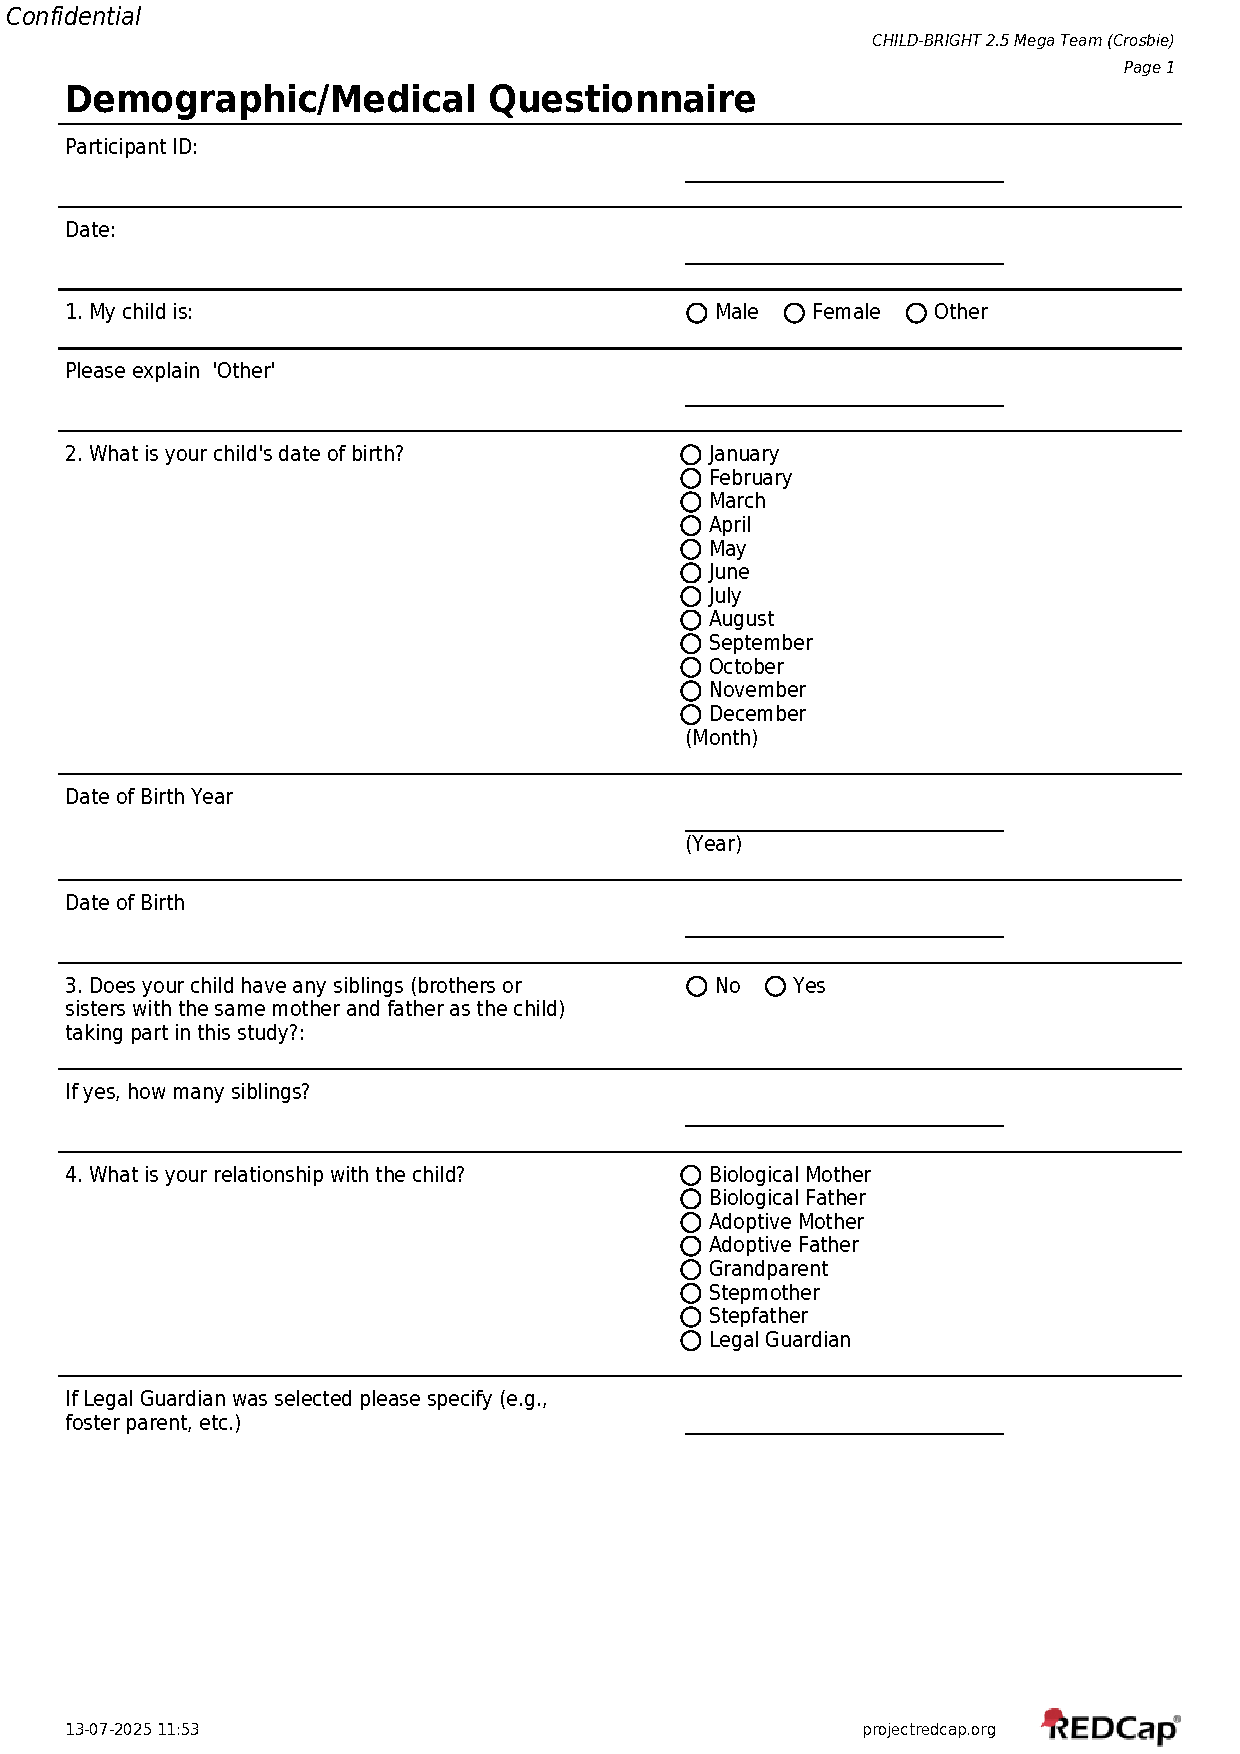
\includepdf[pages=1-4, pagecommand={}, scale = 0.85]{apx-dmq.pdf}




\end{document}
